%\documentclass[a4,semhelv,landscape]{seminar}
\documentclass[landscape]{slides}
%\documentclass[pdf, default, slideBW, nocolorBG]{prosper}
\usepackage[left=0.2cm,top=0.2cm,right=0.2cm,bottom=0.2cm,nohead,nofoot]{geometry}
%\def\everyslide{\sffamily}
%\usepackage{fullpage}
\usepackage{graphicx}
\usepackage[usenames]{color}
%\usepackage{color}
\usepackage{verbatim}
\usepackage{nopageno}
\usepackage{setspace}
%\usepackage{times}
% define some nice colors
\definecolor{myred}{rgb}{0.6,0,0}
\definecolor{myblue}{rgb}{0,0.2,0.4}
\definecolor{mygreen}{rgb}{0,0.5,0.0}
\definecolor{mypurple}{cmyk}{0.5,1.0,0.0,0.0}
%\color{myblue}

\begin{document}
%%%%%%%%%%%%%%%%%%%%%%%%%%%%%%%%%%%%%%%%%%%%%%%%%%%%%%%%%%%%%%%%%%%%
%Slide 0 - title
\begin{slide}
\begin{center}
\large{\textbf{Reference-guided annotation of viral genomes}}

\normalsize

Eric Nawrocki \\

\medskip

\medskip

\medskip

\medskip

\medskip

\small
\begin{tabular}{c}
Alejandro Sch\"{a}ffer's group \\
\\
National Center for Biotechnology Information\\
National Institutes of Health\\
\\
\end{tabular}

\vspace{0.1in}


\includegraphics[width=2.5in]{figs/ncbi-logo}

\end{center}
\end{slide}
%%%%%%%%%%%%%%%%%%%%%%%%%%%%%%%%%%%%%%%%%%%%%%%%%%%%%%%%%%%%%%%%%%%%%%
\begin{slide}
\begin{center}

\textbf{Most prevalent viral genomes in GenBank\footnote{Influenza is omitted.}}

\tiny
\begin{tabular}{r|l|r|l|l|l|r|r}
       &                    &              &                &          &        &       & \#mature \\ 
  rank & species            &       \#seqs & family         & type     & host   & \#cds & peptides \\ \hline
       &                    &              &                &          &        &       &          \\ 
     1 & Hepatitis B        &         7061 & Hepadnaviridae & dsDNA-RT & humans &     7 &       -  \\
       &                    &              &                &          &        &       &          \\ 
     2 & Dengue             &         3875 & Flaviviridae   & (+)ssRNA & humans &     1 &      14  \\
       &                    &              &                &          &        &       &          \\ 
     3 & Rotavirus          &      22536\footnote{sum of 11 segments}  & Reoviridae     & dsRNA    & humans &    12 &       -  \\
       &                    &              &                &          &        &       &          \\ 
     4 & HIV-1              &        2132  & Retroviridae   & ssRNA-RT & humans &    10 &      14  \\
       &                    &              &                &          &        &       &          \\ 
     5 & Porcine circovirus &        1559  & Circoviridae   & ssDNA    & pigs   &     3 &       -  \\
       &                    &              &                &          &        &       &          \\ 
     6 & Hepatitis C        &        1457  & Flaviviridae   & (+)ssRNA & humans &     2 &      10  \\
       &                    &              &                &          &        &       &          \\ 
     7 & West Nile          &        1109  & Flaviviridae   & (+)ssRNA & humans &     3 &      16  \\
       &                    &              &                &          &        &       &          \\ 
     8 & Ebola              &        1105  & Flaviviridae   & (+)ssRNA & humans &     9 &       -  \\
       &                    &              &                &          &        &       &          \\ 
     9 & Enterovirus A      &         932  & Picarnoviridae & (+)ssRNA & humans &     1 &      11  \\
       &                    &              &                &          &        &       &          \\ 
    10 & RSV                &         623  & Paramyxoviridae& (-)ssRNA & humans &    11 &       -  \\
       &                    &              &                &          &        &       &          \\ 
    11 & Enterovirus C (Polio) &      618  & Picarnoviridae & (+)ssRNA & humans &     1 &      13  \\
       &                    &              &                &          &        &       &          \\ 
    12 & JC polyomavirus    &          598 & Polyomaviridae & dsDNA    & humans &     6 &       -  \\
       &                    &              &                &          &        &       &          \\ 
    13 & PRRSV              &          520 & Arteriviridae  & (+)ssRNA & pigs   &    11 &      13  \\ %# 15 mat_peptide segments, 13 mat_peptides 
       &                    &              &                &          &        &       &          \\ 
    14 & Maize streak virus &          508 & Geminiviridae  & ssDNA    & plants &     4 &      -   \\
       &                    &              &                &          &        &       &          \\ 
    15 & Norwalk virus      &          491 &  Calciviridae  & (+)ssRNA & humans &     3 &       6  \\ 
\end{tabular}

% SAME TABLE, WITH EXON COUNTS
%\tiny
%\begin{tabular}{r|l|r|l|l|l|r|r|r}
%       &                    &              &                &          &        &       &        & mature   \\ 
%   rank& species            &     \# seqs & family         & type     & host   & \#cds &\#exons & peptides \\ \hline
%     1 & Hepatitis B        &        7061 & Hepadnaviridae  & dsDNA-RT & humans &     7 &      7 &       -  \\
%     2 & Dengue             &        3875 & Flaviviridae    & (+)ssRNA & humans &     1 &      1 &      14  \\
%     3 & Rotavirus          &      22536* & Reoviridae      & dsRNA    & humans &    12 &      ? &       -  \\
%     4 & HIV-1              &        2132 & Retroviridae    & ssRNA-RT & humans &    10 &     14 &      14  \\
%     5 & Porcine circovirus &        1559 & Circoviridae    & ssDNA    & pigs   &     3 &      3 &       -  \\
%     6 & Hepatitis C        &        1457 & Flaviviridae    & (+)ssRNA & humans &     2 &      3 &      10  \\
%     7 & West Nile          &       2218* & Flaviviridae    & (+)ssRNA & humans &     3 &      5 &      16  \\
%     8 & Ebola              &        1105 & Flaviviridae    & (+)ssRNA & humans &     9 &     11 &       -  \\
%     9 & Enterovirus A      &         932 & Picarnoviridae  & (+)ssRNA & humans &     1 &      1 &      11  \\
%    10 & RSV                &         623 & Paramyxoviridae & (-)ssRNA & humans &    11 &     11 &       -  \\
%    11 & Enterovirus C (Polio) &      618 & Picarnoviridae  & (+)ssRNA & humans &     1 &      1 &      13  \\
%    12 & JC polyomavirus   &          598 & Polyomaviridae  & dsDNA    & humans &     6 &      7 &       -  \\
%    13 & PRRSV             &          520 & Arteriviridae   & (+)ssRNA & pigs   &    11 &     13 &  13(15)  \\ %# 15 mat_peptide segments, 13 mat_peptides 
%    14 & Maize streak virus&          508 & Geminiviridae   & ssDNA    & plants &     4 &      5 &      -   \\
%    15 & Norwalk virus     &          491 &  Calciviridae   & (+)ssRNA & humans &     3 &      3 &      6   \\ 
%\end{tabular}

\end{center}
\tiny
\flushright{$\dagger$ sum of 11 segments}
\vfill

\end{slide}
%%%%%%%%%%%%%%%%%%%%%%%%%%%%%%%%%%%%%%%%%%%%%%%%%%%%%%%%%%%%%%%%%%%%%%
\begin{slide}
\begin{center}
\textbf{The Virus Variation Resource is a powerful tool for viral research}

\begin{minipage}[c]{4in}
\tiny
\begin{itemize}
\item value added database that includes annotations not in GenBank
\item allows users to: 
\begin{itemize}
  \item select subsets of data based on desired criteria
    (host, country, gene, etc.)
  \item download alignments
  \item  compute trees
  \item  more...
\end{itemize}
\end{itemize}
\vfill
\end{minipage}
\begin{minipage}[c]{6in}
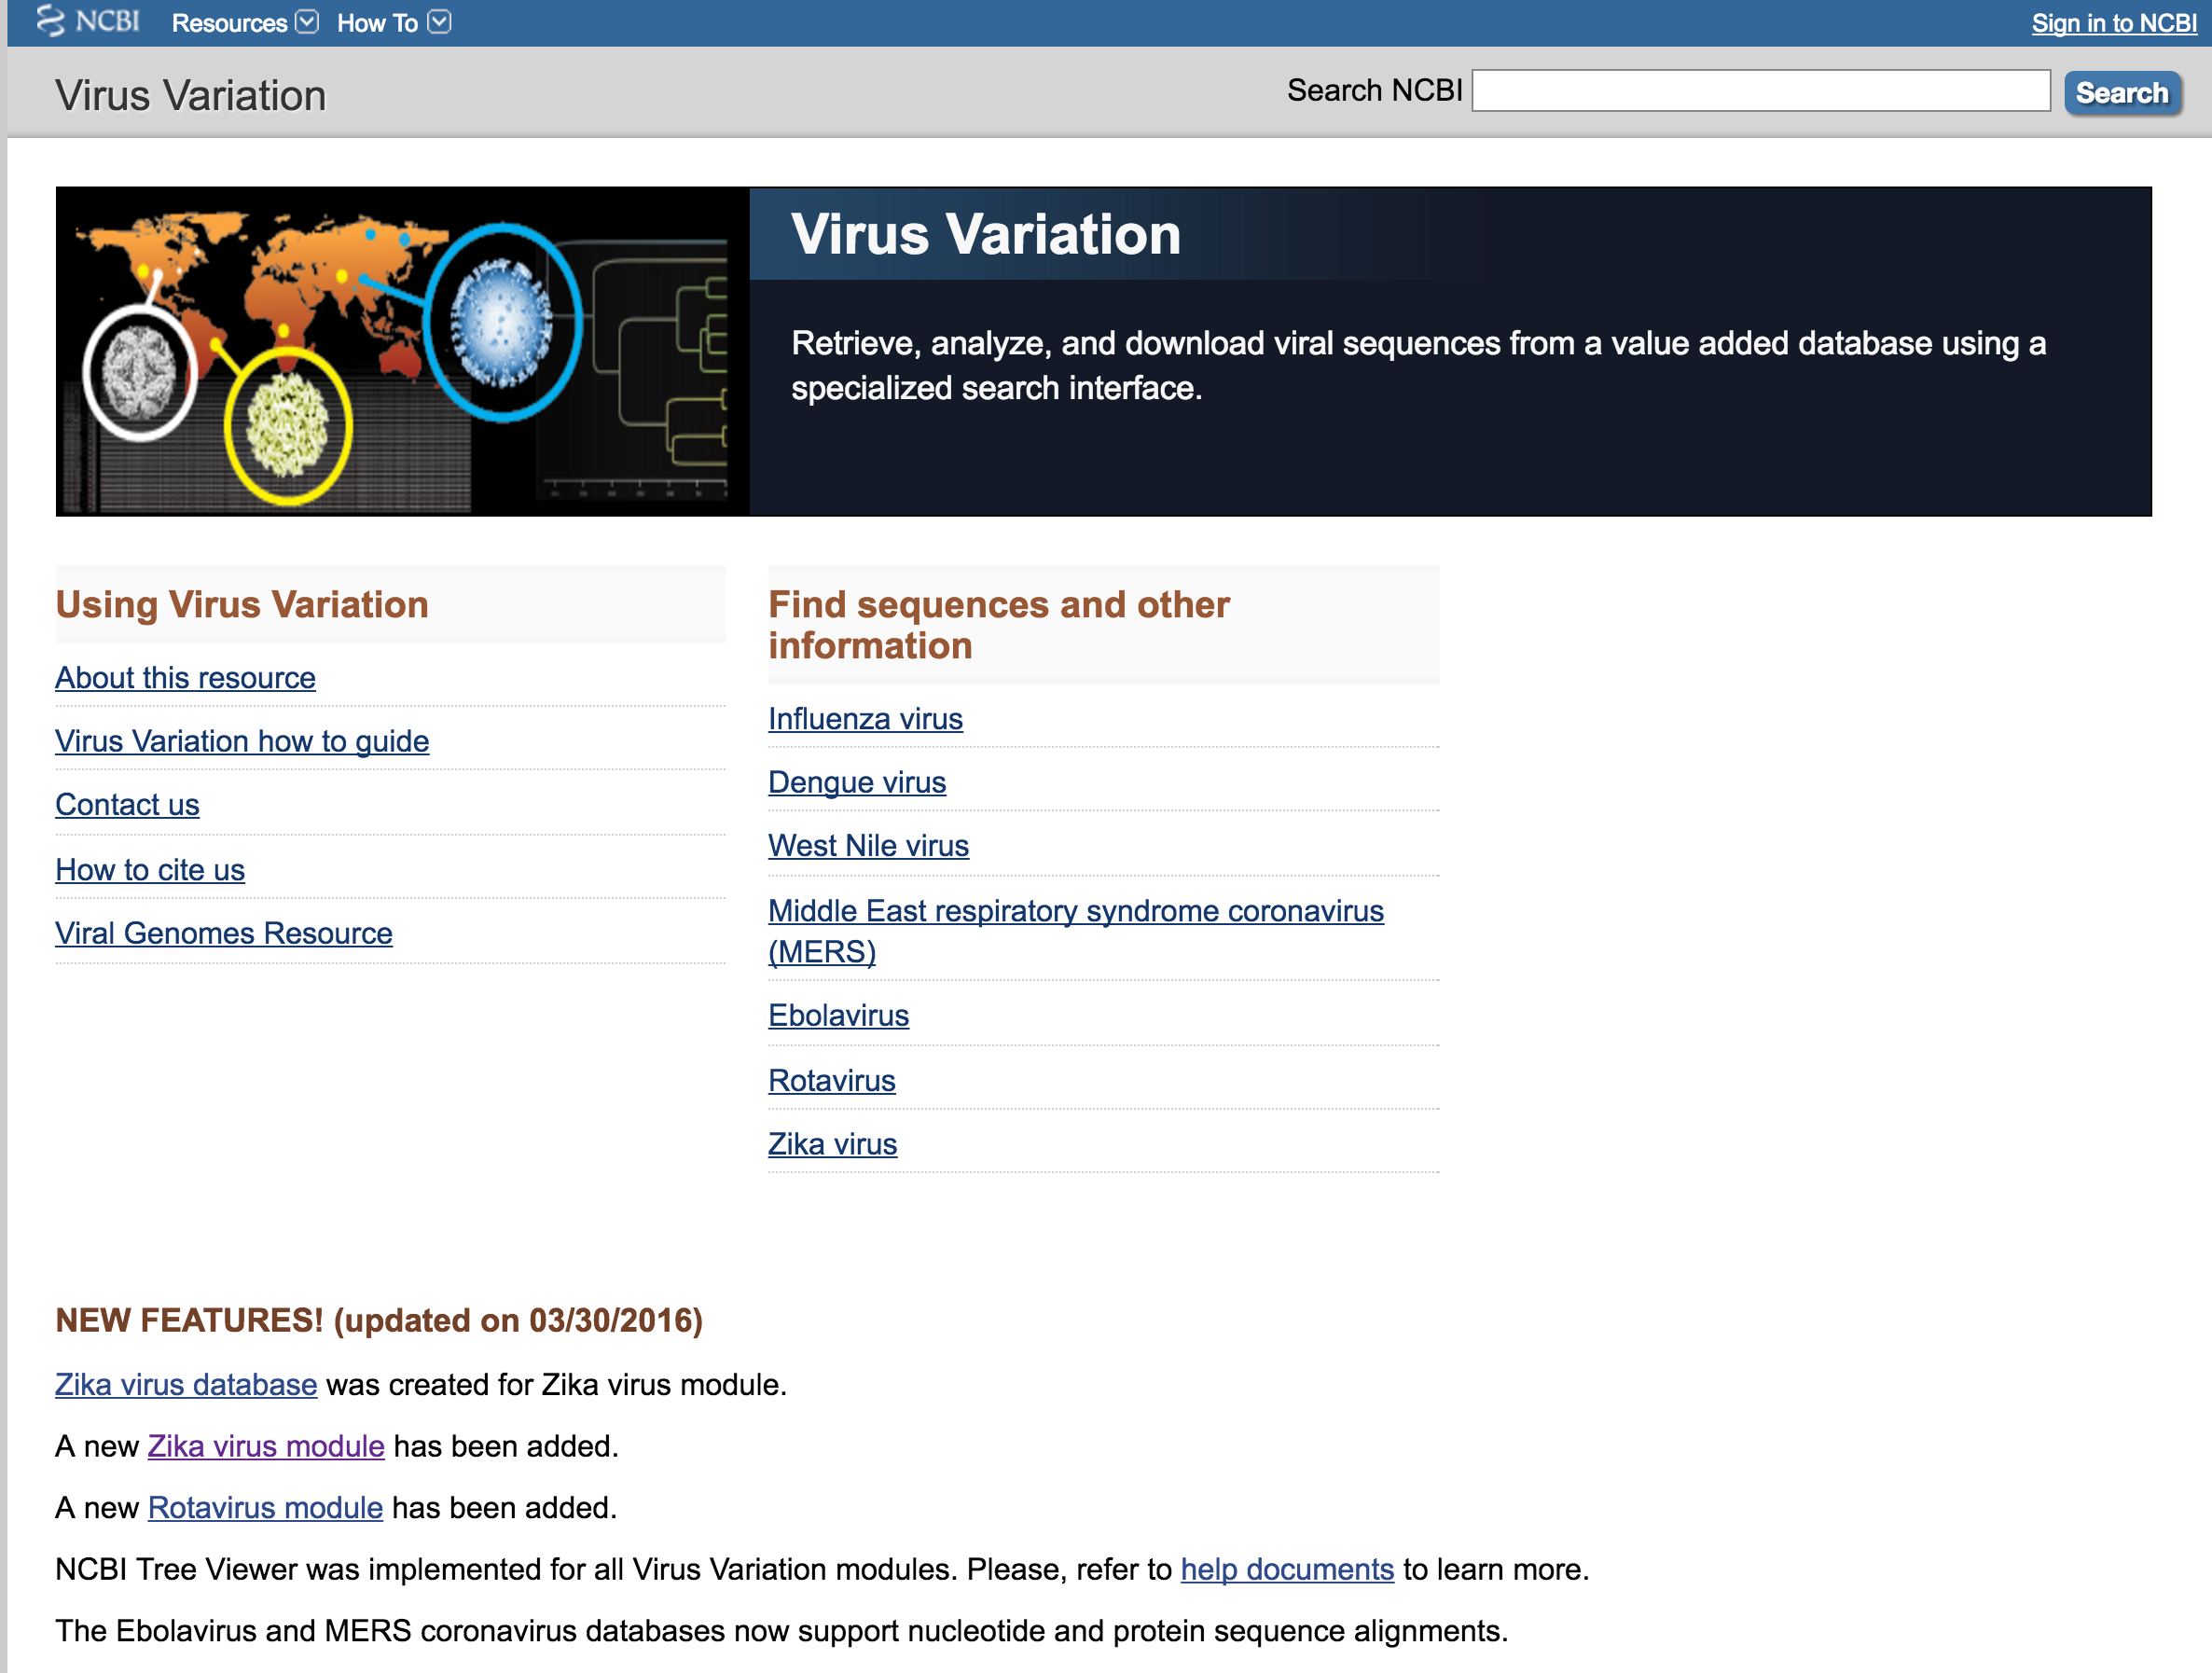
\includegraphics[width=6in]{figs/viv-page1}
\vfill
\end{minipage}

\vfill
\end{center}
\end{slide}
%%%%%%%%%%%%%%%%%%%%%%%%%%%%%%%%%%%%%%%%%%%%%%%%%%%%%%%%%%%%%%%%%%%%%%
\begin{slide}
\begin{center}
\textbf{The Virus Variation Resource is a powerful tool for viral research}

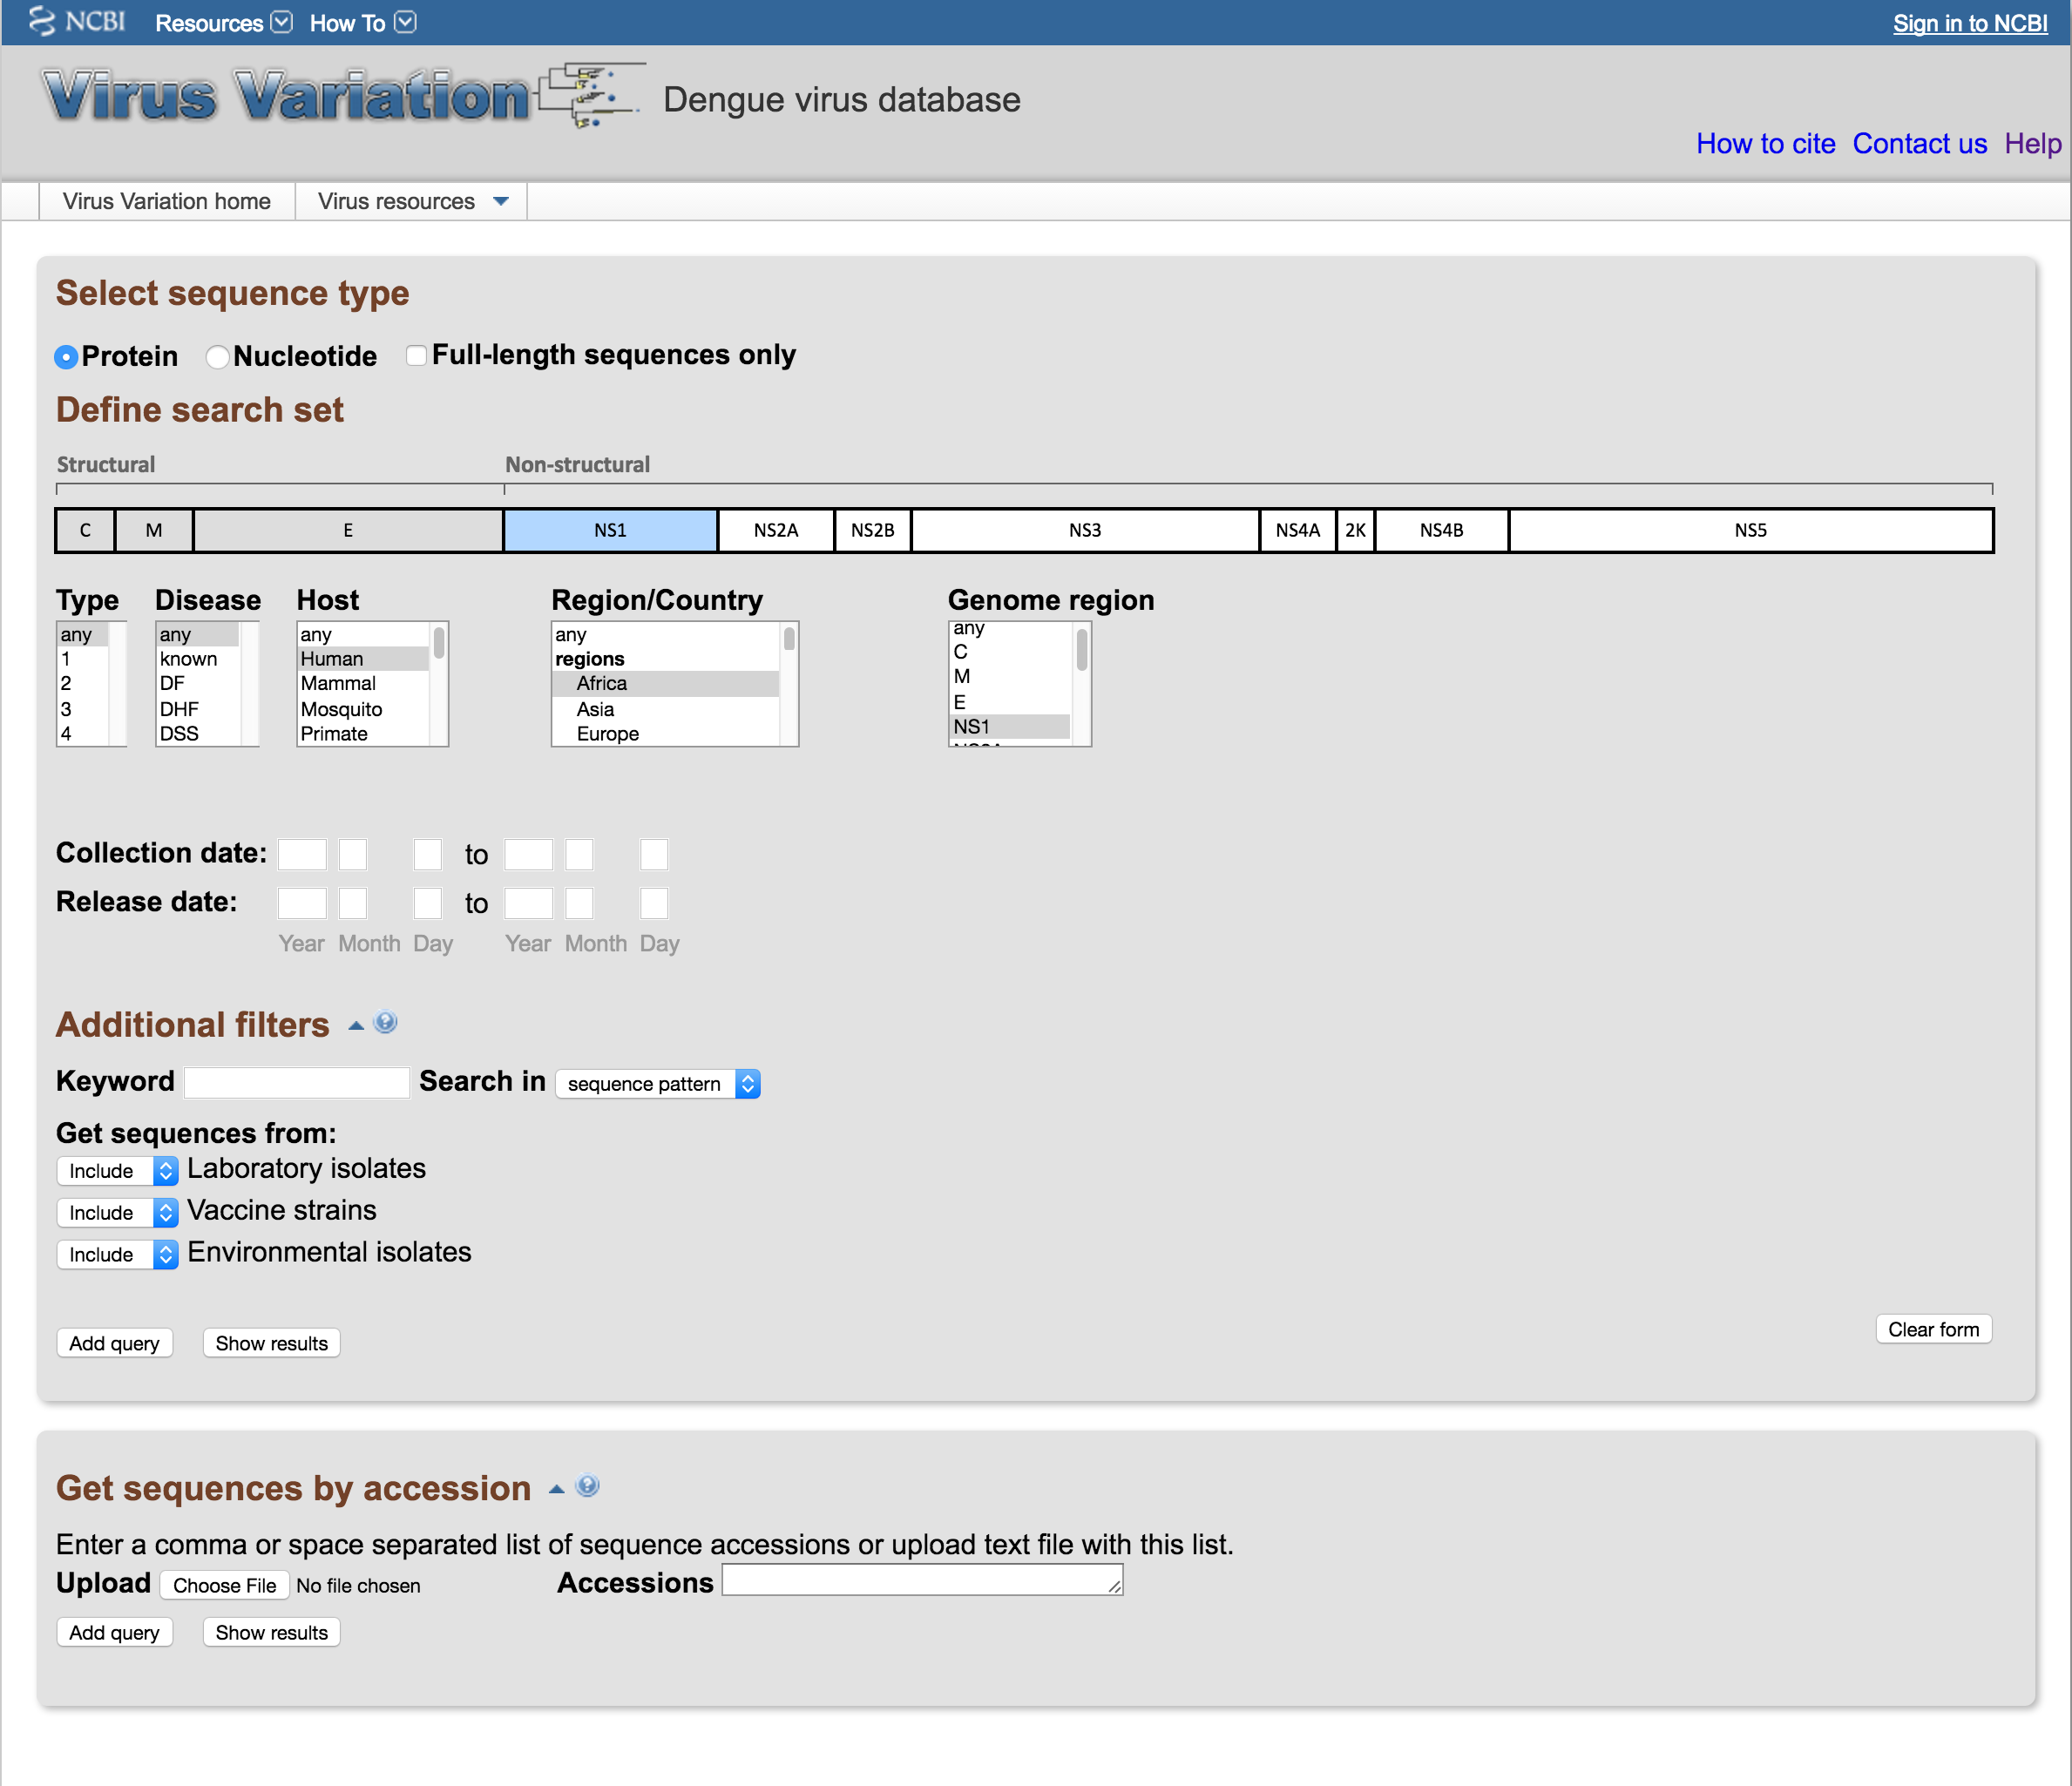
\includegraphics[width=8in]{figs/viv-dengue-query}

\vfill
\end{center}
\end{slide}
%%%%%%%%%%%%%%%%%%%%%%%%%%%%%%%%%%%%%%%%%%%%%%%%%%%%%%%%%%%%%%%%%%%%%%
\begin{slide}
\begin{center}
\textbf{Our goal is to develop an annotation pipeline to benefit \\ Virus Variation}

\small
\begin{itemize}
\item general method for annotating existing and new viral genome
  sequences for a species using trusted annotation for that species (e.g. RefSeq)
\item identify interesting characteristics that Viral Variation can
  allow users to sort/select based on:
\begin{itemize}
  \item identification of high quality sequences that meet specific expectations
  \item identification of sequences that deviate from expectations
  \item full or partial length
  \item fractional identity to reference
  \item more...
\end{itemize}
\end{itemize}

\end{center}
\vfill
\end{slide}
%%%%%%%%%%%%%%%%%%%%%%%%%%%%%%%%%%%%%%%%%%%%%%%%%%%%%%%%%%%%%%%%%%%%%%
% 
% Pilot species:
%%%%%%%%%%%%%%%%%%%%%%%%%%%%%%%%%%%%%%%%%%%%%%%%%%%%%%%%%%%%%%%%%%%%%%
\begin{slide}
\begin{center}

\textbf{Four pilot species were chosen from the 15 most prevalent}

\tiny
\begin{tabular}{r|l|r|l|l|l|r|r}
       &                    &              &                &          &        &       & \#mature \\ 
  rank & species            &       \#seqs & family         & type     & host   & \#cds & peptides \\ \hline
       &                    &              &                &          &        &       &          \\ 
\textcolor{red}{1} & \textcolor{red}{Hepatitis B}        &         \textcolor{red}{7061} & \textcolor{red}{Hepadnaviridae} & \textcolor{red}{dsDNA-RT} & \textcolor{red}{humans} &     \textcolor{red}{7} &       \textcolor{red}{-}  \\
       &                    &              &                &          &        &       &          \\ 
\textcolor{red}{2} & \textcolor{red}{Dengue}             &         \textcolor{red}{3875} & \textcolor{red}{Flaviviridae}   & \textcolor{red}{(+)ssRNA} & \textcolor{red}{humans} &     \textcolor{red}{1} &      \textcolor{red}{14}  \\
       &                    &              &                &          &        &       &          \\ 
     3 & Rotavirus          &      22536*  & Reoviridae     & dsRNA    & humans &    12 &       -  \\
       &                    &              &                &          &        &       &          \\ 
     4 & HIV-1              &        2132  & Retroviridae   & ssRNA-RT & humans &    10 &      14  \\
       &                    &              &                &          &        &       &          \\ 
     5 & Porcine circovirus &        1559  & Circoviridae   & ssDNA    & pigs   &     3 &       -  \\
       &                    &              &                &          &        &       &          \\ 
     \textcolor{red}{6} & \textcolor{red}{West Nile}          &        \textcolor{red}{1109} & \textcolor{red}{Flaviviridae}   & \textcolor{red}{(+)ssRNA} & \textcolor{red}{humans} &     \textcolor{red}{3} &      \textcolor{red}{16}  \\
       &                    &              &                &          &        &       &          \\ 
     7 & Hepatitis C        &        1457  & Flaviviridae   & (+)ssRNA & humans &     2 &      10  \\
       &                    &              &                &          &        &       &          \\ 
     8 & Ebola              &        1105  & Flaviviridae   & (+)ssRNA & humans &     9 &       -  \\
       &                    &              &                &          &        &       &          \\ 
     9 & Enterovirus A      &         932  & Picarnoviridae & (+)ssRNA & humans &     1 &      11  \\
       &                    &              &                &          &        &       &          \\ 
    10 & RSV                &         623  & Paramyxoviridae& (-)ssRNA & humans &    11 &       -  \\
       &                    &              &                &          &        &       &          \\ 
    11 & Enterovirus C (Polio) &      618  & Picarnoviridae & (+)ssRNA & humans &     1 &      13  \\
       &                    &              &                &          &        &       &          \\ 
    12 & JC polyomavirus    &          598 & Polyomaviridae & dsDNA    & humans &     6 &       -  \\
       &                    &              &                &          &        &       &          \\ 
    13 & PRRSV              &          520 & Arteriviridae  & (+)ssRNA & pigs   &    11 &      13  \\ %# 15 mat_peptide segments, 13 mat_peptides 
       &                    &              &                &          &        &       &          \\ 
    \textcolor{red}{14} & \textcolor{red}{Maize streak virus} &          \textcolor{red}{508} & \textcolor{red}{Geminiviridae}  & \textcolor{red}{ssDNA}    & \textcolor{red}{plants} &     \textcolor{red}{4} &      \textcolor{red}{-}   \\
       &                    &              &                &          &        &       &          \\ 
    15 & Norwalk virus      &          491 &  Calciviridae  & (+)ssRNA & humans &     3 &       6  \\ 
\end{tabular}

\end{center}

\tiny
\flushright{$\dagger$ sum of 11 segments}
\vfill
\end{slide}
%%%%%%%%%%%%%%%%%%%%%%%%%%%%%%%%%%%%%%%%%%%%%%%%%%%%%%%%%%%%%%%%%%%%%%
\begin{slide}
\begin{center}
\textbf{Maize Streak Virus}

\begin{minipage}[c]{6in}
\tiny
\begin{itemize}
\item cause of most serious crop disease in Africa, responsible for
  between USD\$100-\$500 million of crop loss per year
\item NC\_001346 (2689 nt):
  \begin{itemize}
    \item 4 CDS (V1, V2, C1, C1:C2), 5 total ‘exons’
    \item both strands have $>=$ 1 CDS
    \item one CDS (C1:C2) has two segments (exons)
    \item origin sequence: TAATATT$|$AC
  \end{itemize}
\item circular genome
\item 508 full genome sequences in GenBank
\begin{itemize}
  \item average number of CDS annotated: 3.34
%  \item average number of exons annotated: ?
\end{itemize}
\end{itemize}
\vspace{3in}
\end{minipage}
\begin{minipage}[c]{4in}
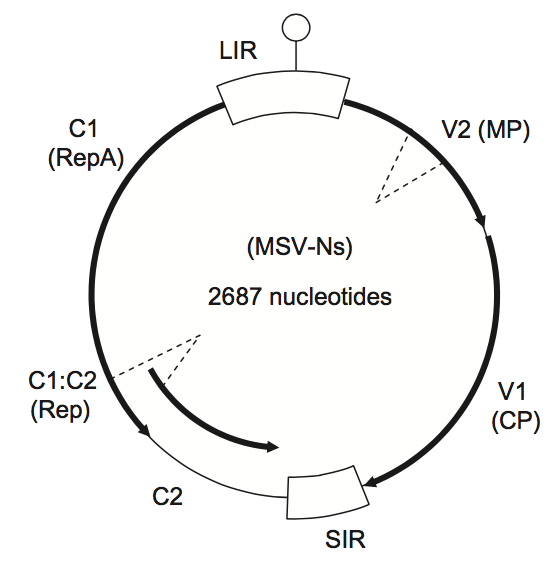
\includegraphics[width=4in]{figs/msv-genome-small}
\vspace{3in}
\end{minipage}

\vfill
\end{center}
\end{slide}
%%%%%%%%%%%%%%%%%%%%%%%%%%%%%%%%%%%%%%%%%%%%%%%%%%%%%%%%%%%%%%%%%%%%%%
\begin{slide}
\begin{center}
\textbf{Dengue virus}

\small
\begin{itemize}
\item up to 400 million people infected per year worldwide
\item a single CDS encodes the flavivirus polyprotein gene
\item the polyprotein is cleaved into 14 smaller 'mature peptides'
\item annotations exist in Virus Variation to compare against our own
\end{itemize}

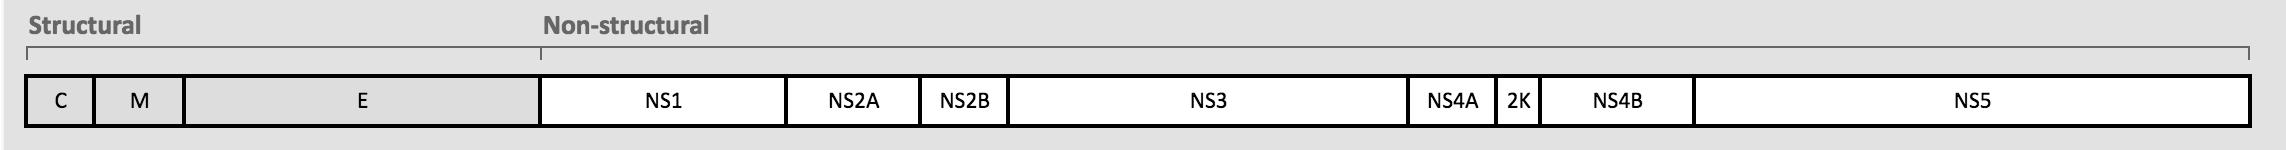
\includegraphics[width=9.5in]{figs/dengue-genome-organization}

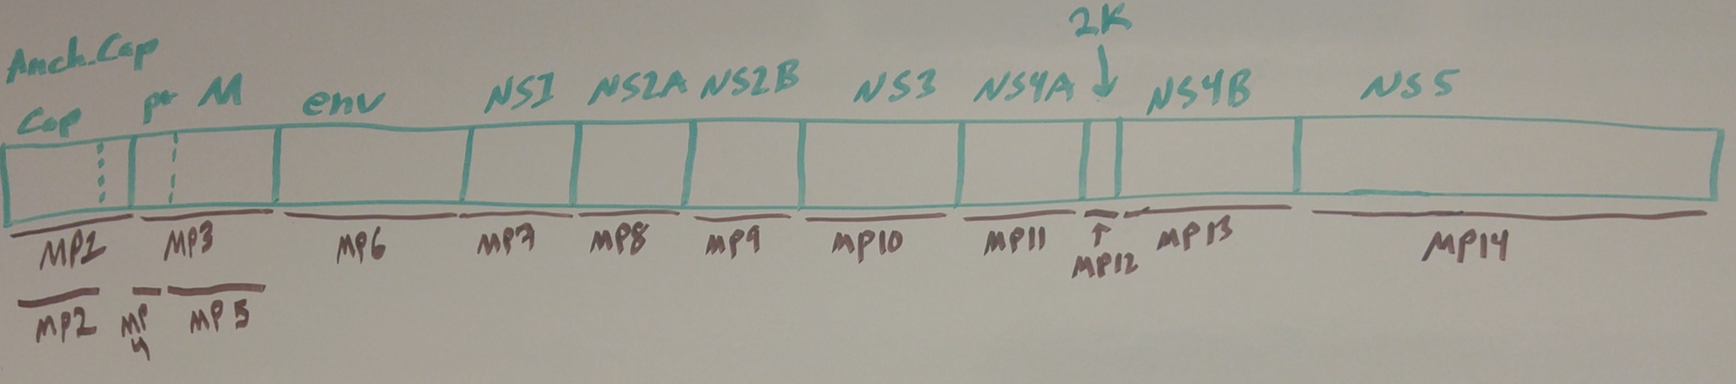
\includegraphics[width=9.5in]{figs/dengue-eneida}\footnote{illustration
  by Eneida Hatcher}


\end{center}
\vfill
\end{slide}
%%%%%%%%%%%%%%%%%%%%%%%%%%%%%%%%%%%%%%%%%%%%%%%%%%%%%%%%%%%%%%%%%%%%%%
\begin{slide}
\begin{center}
\textbf{West Nile virus}

\small  
\begin{itemize}
\item another flavivirus, similar to Dengue
\item 3 CDS, including:
\begin{itemize}
  \item two CDS that utilize ribosomal frameshift to change reading
    frame, \\ possibly complicating annotation
\item West Nile annotations do not yet exist in Virus Variation
\end{itemize}
\end{itemize}

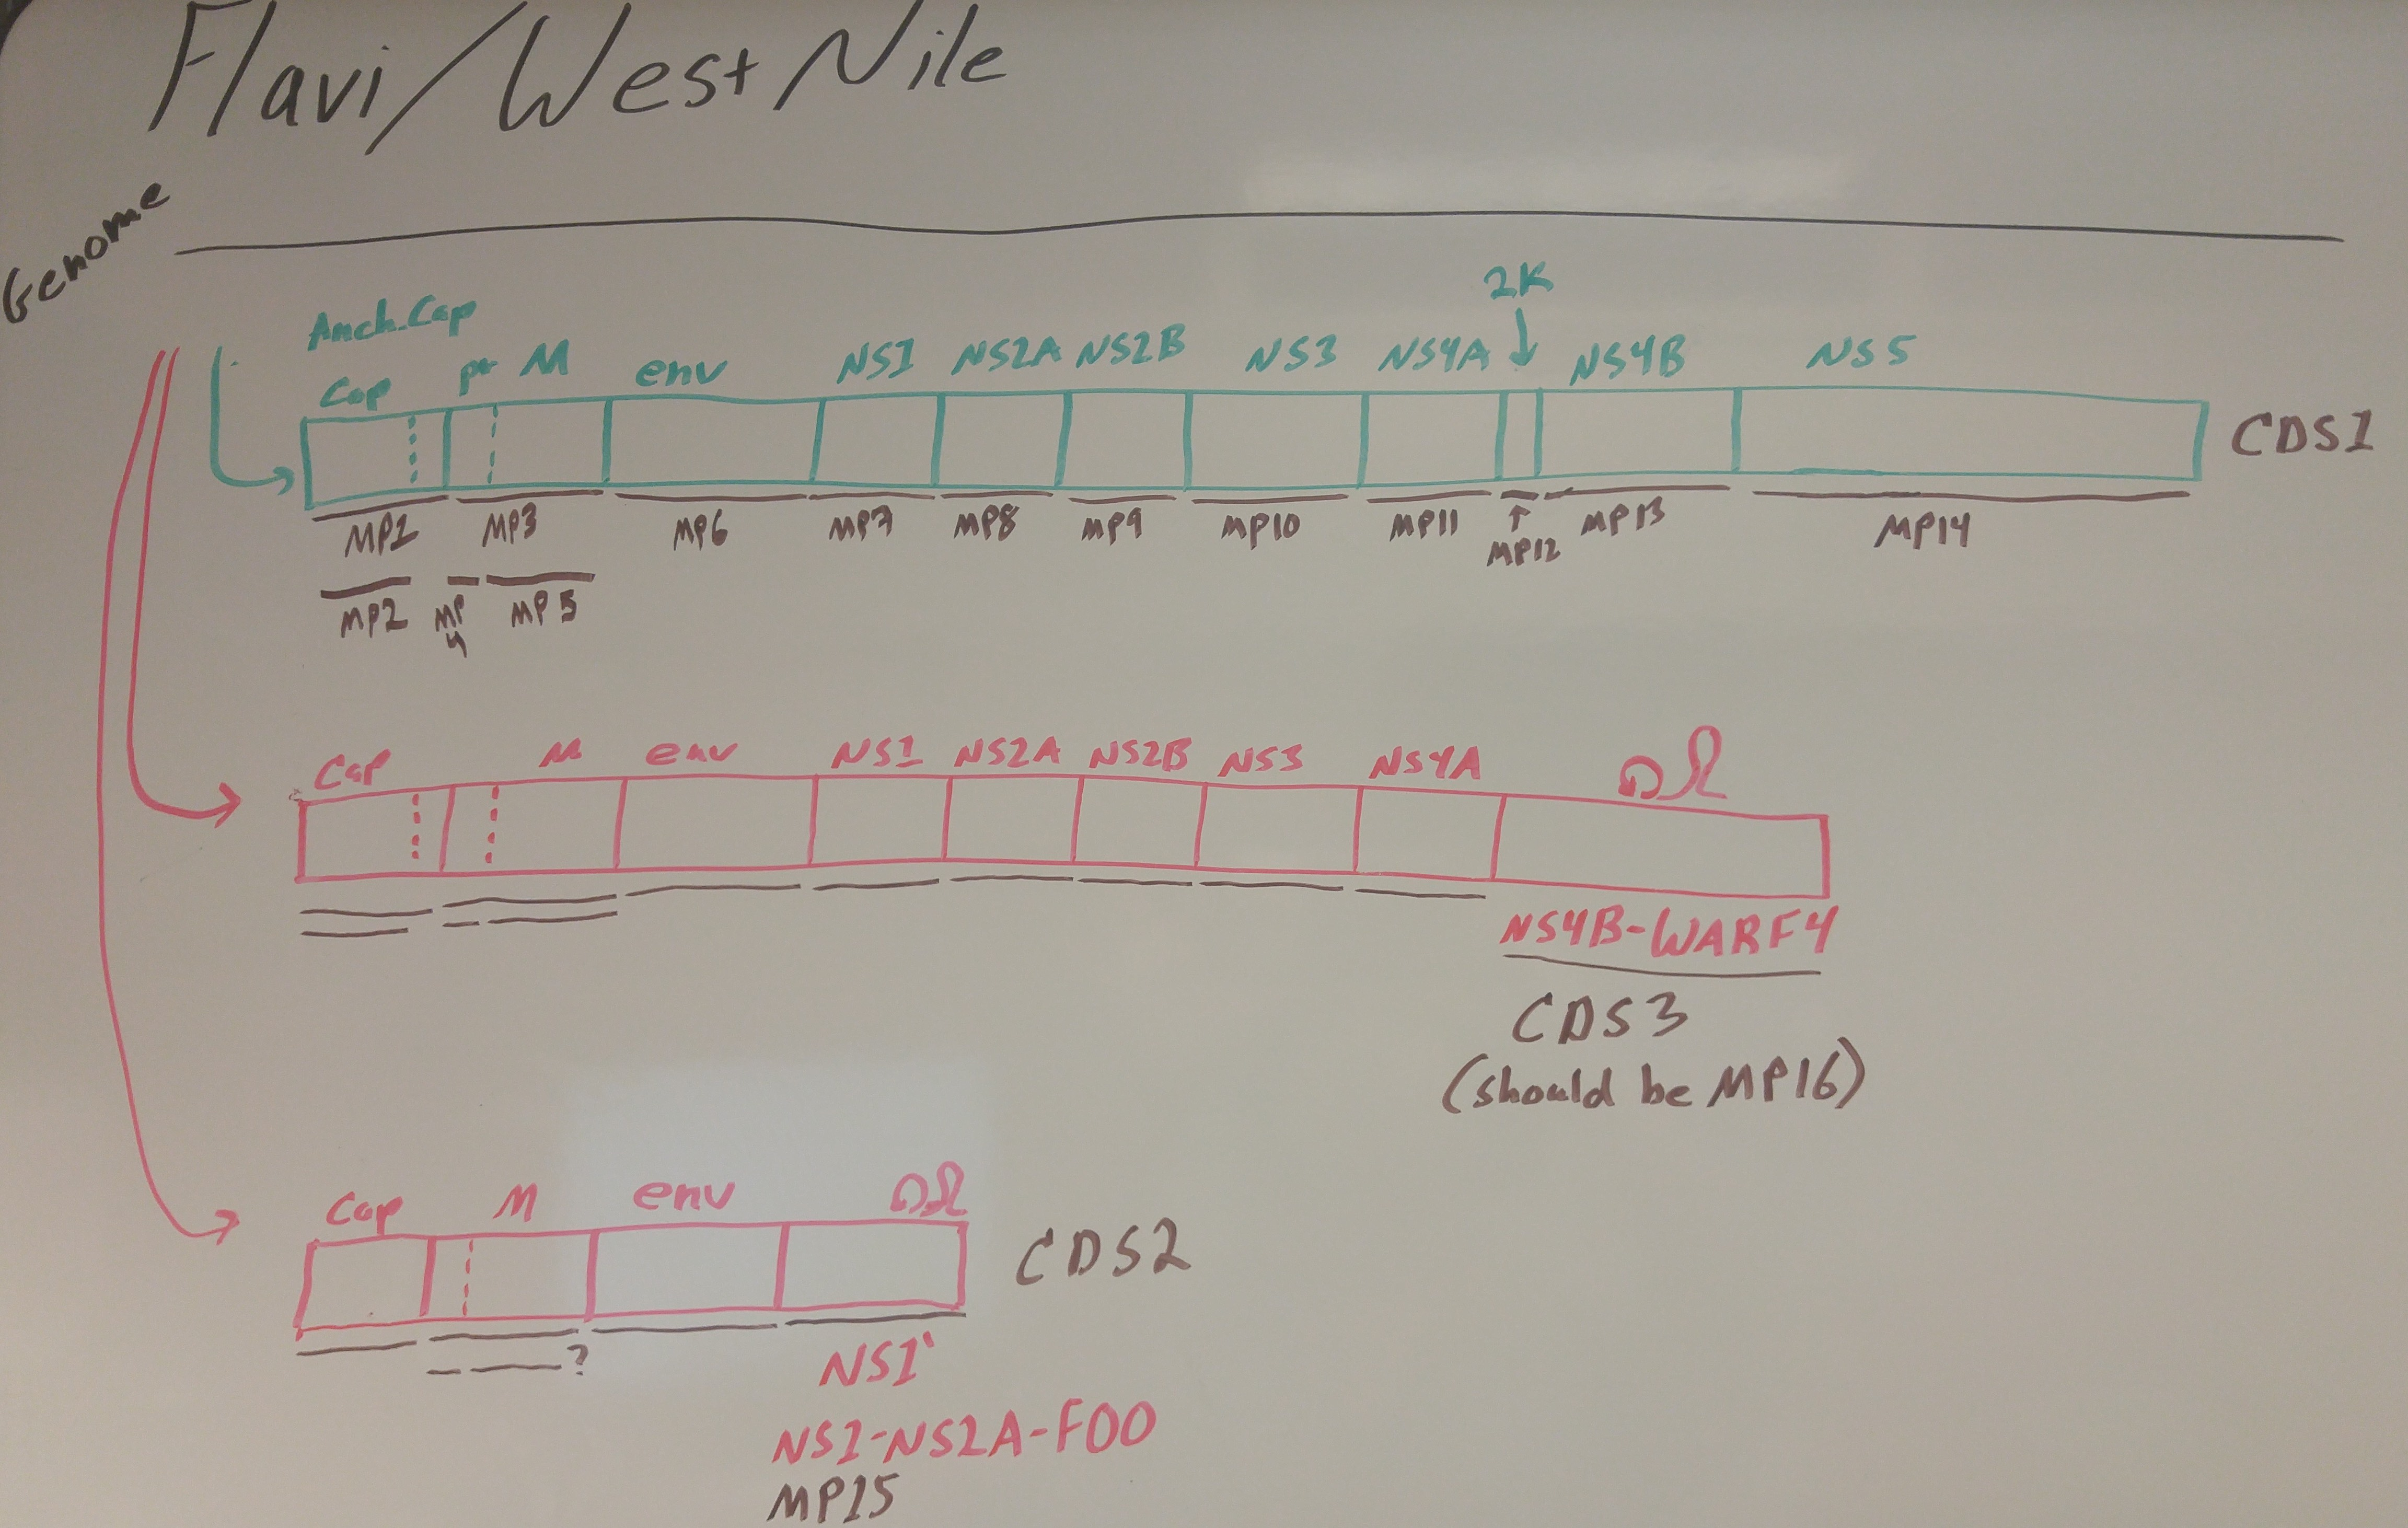
\includegraphics[width=8in]{figs/flavi-wnv-eneida}\footnote{illustration
  by Eneida Hatcher}

\end{center}
\vfill

\end{slide}
%%%%%%%%%%%%%%%%%%%%%%%%%%%%%%%%%%%%%%%%%%%%%%%%%%%%%%%%%%%%%%%%%%%%%%
\begin{slide}
\begin{center}
\textbf{Hepatitis B virus}

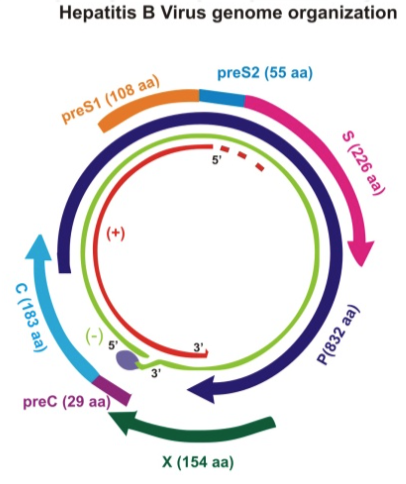
\includegraphics[height=6in]{figs/hbv-genome}

\begin{itemize}
\item non-flu virus with most full length sequences in GenBank
\item circular genome like MSV
\item circular genome like MSV
\end{itemize}

\vfill
\end{center}
\end{slide}
%%%%%%%%%%%%%%%%%%%%%%%%%%%%%%%%%%%%%%%%%%%%%%%%%%%%%%%%%%%%%%%%%%%%%%
\begin{slide}
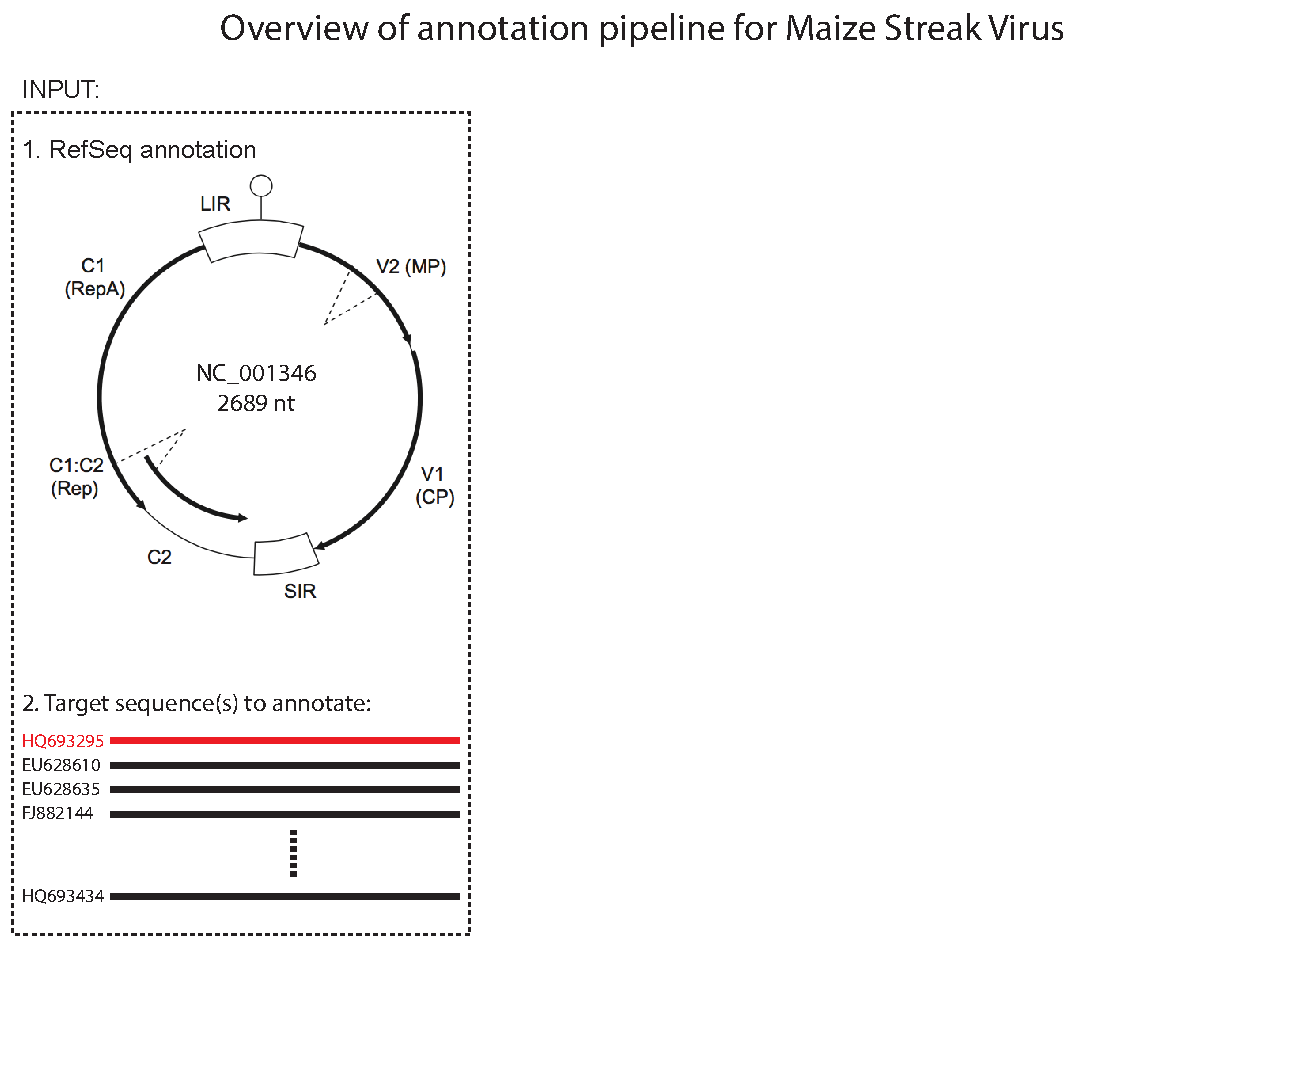
\includegraphics[width=10in]{figs/annotation-schematic-msv-1}
\vfill
\end{slide}
%%%%%%%%%%%%%%%%%%%%%%%%%%%%%%%%%%%%%%%%%%%%%%%%%%%%%%%%%%%%%%%%%%%%%%
\begin{slide}
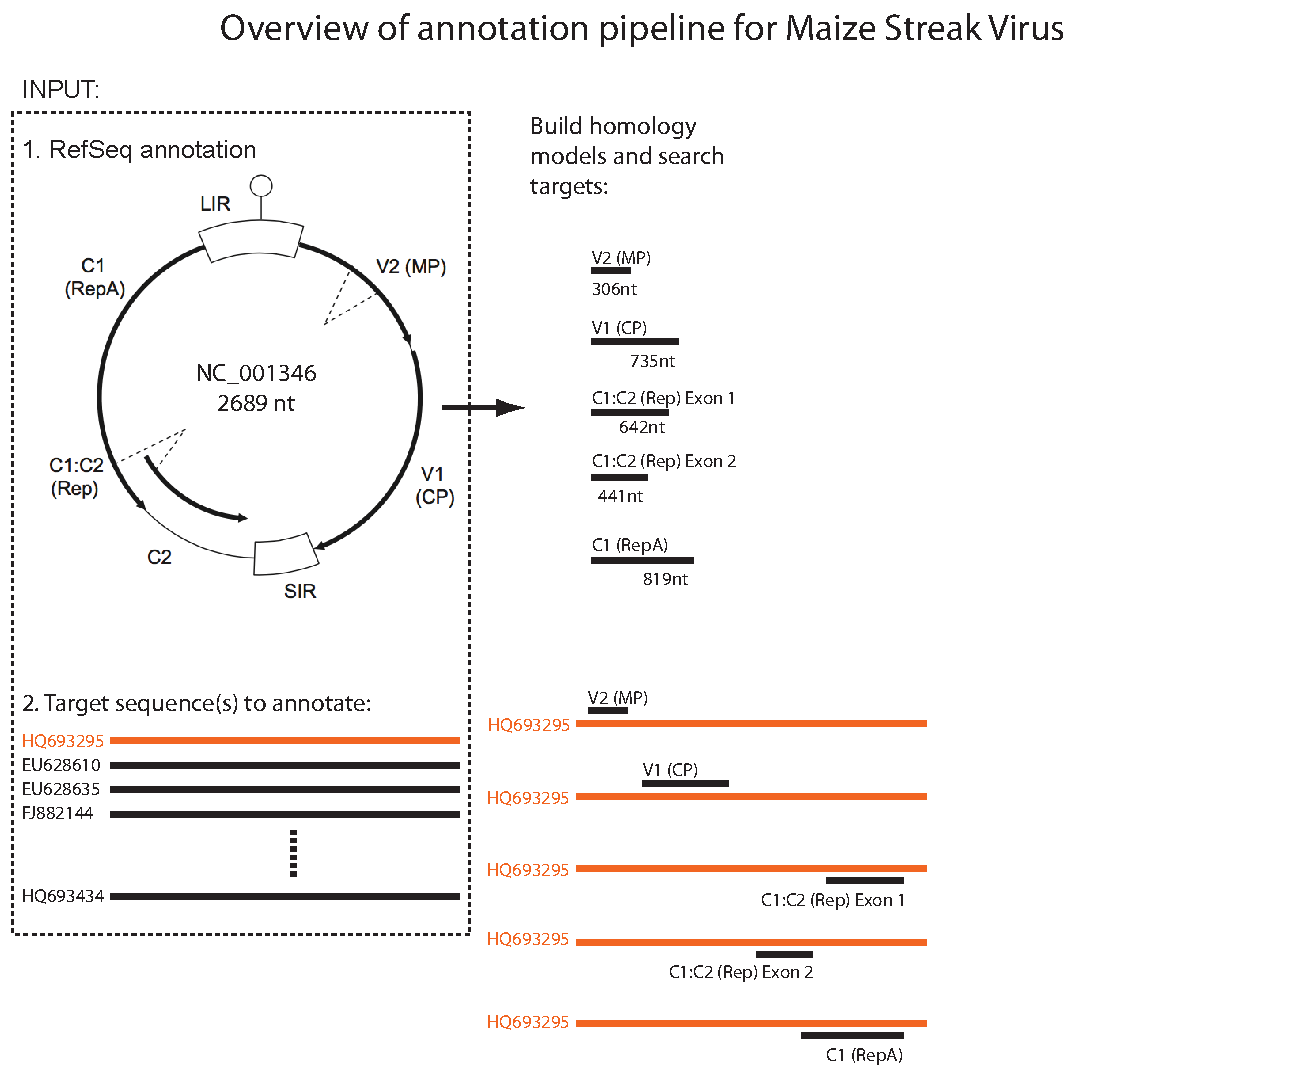
\includegraphics[width=10in]{figs/annotation-schematic-msv-2}
\vfill
\end{slide}
%%%%%%%%%%%%%%%%%%%%%%%%%%%%%%%%%%%%%%%%%%%%%%%%%%%%%%%%%%%%%%%%%%%%%%
\begin{slide}
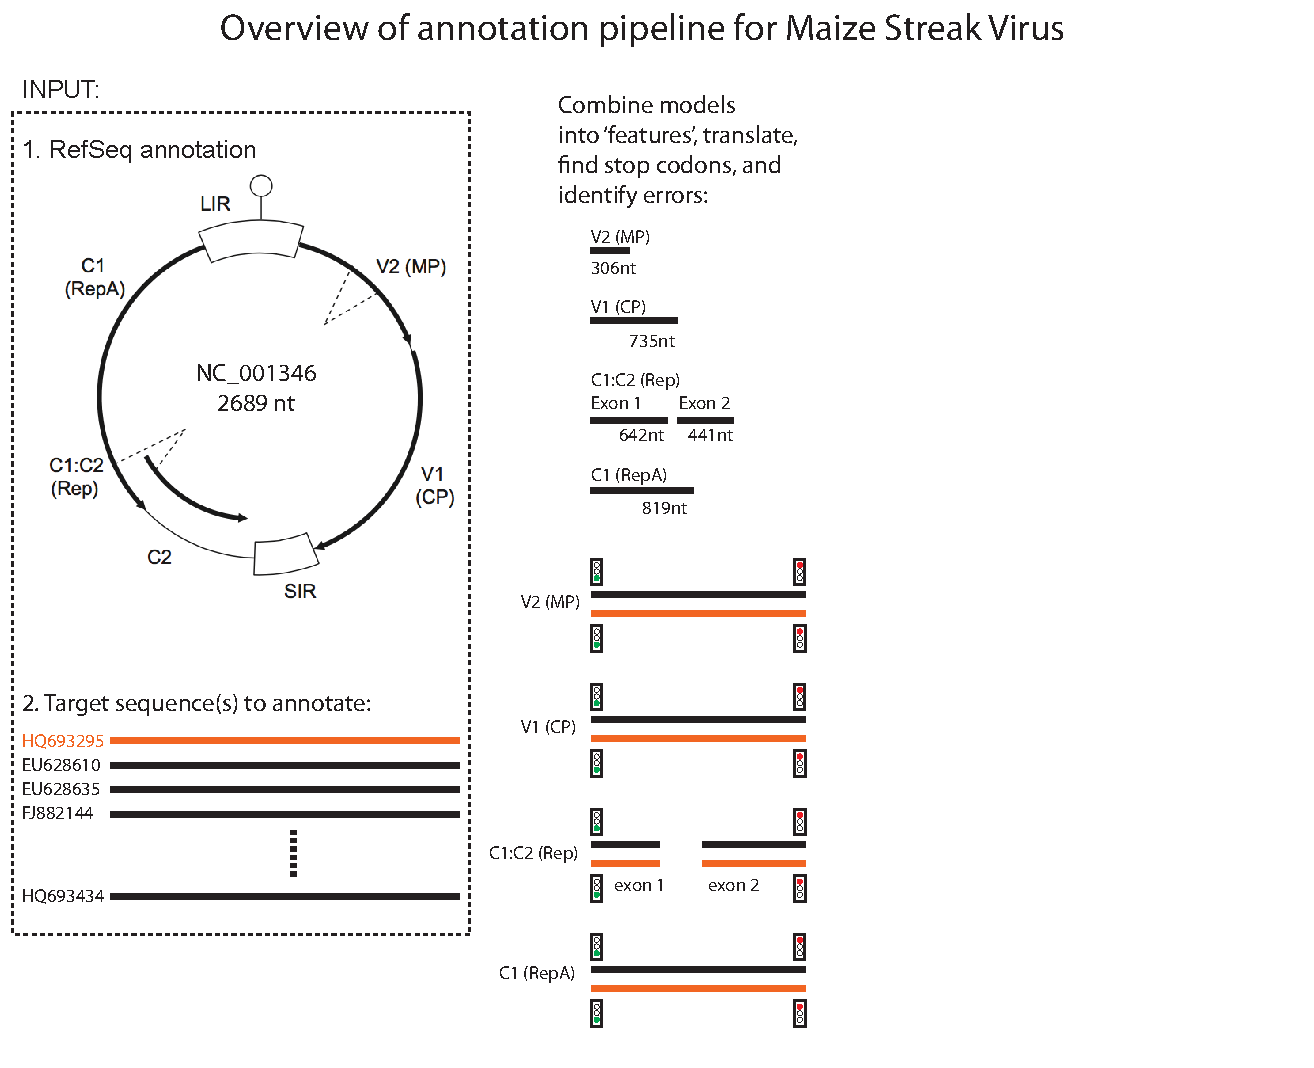
\includegraphics[width=10in]{figs/annotation-schematic-msv-3}
\vfill
\end{slide}
%%%%%%%%%%%%%%%%%%%%%%%%%%%%%%%%%%%%%%%%%%%%%%%%%%%%%%%%%%%%%%%%%%%%%%
\begin{slide}
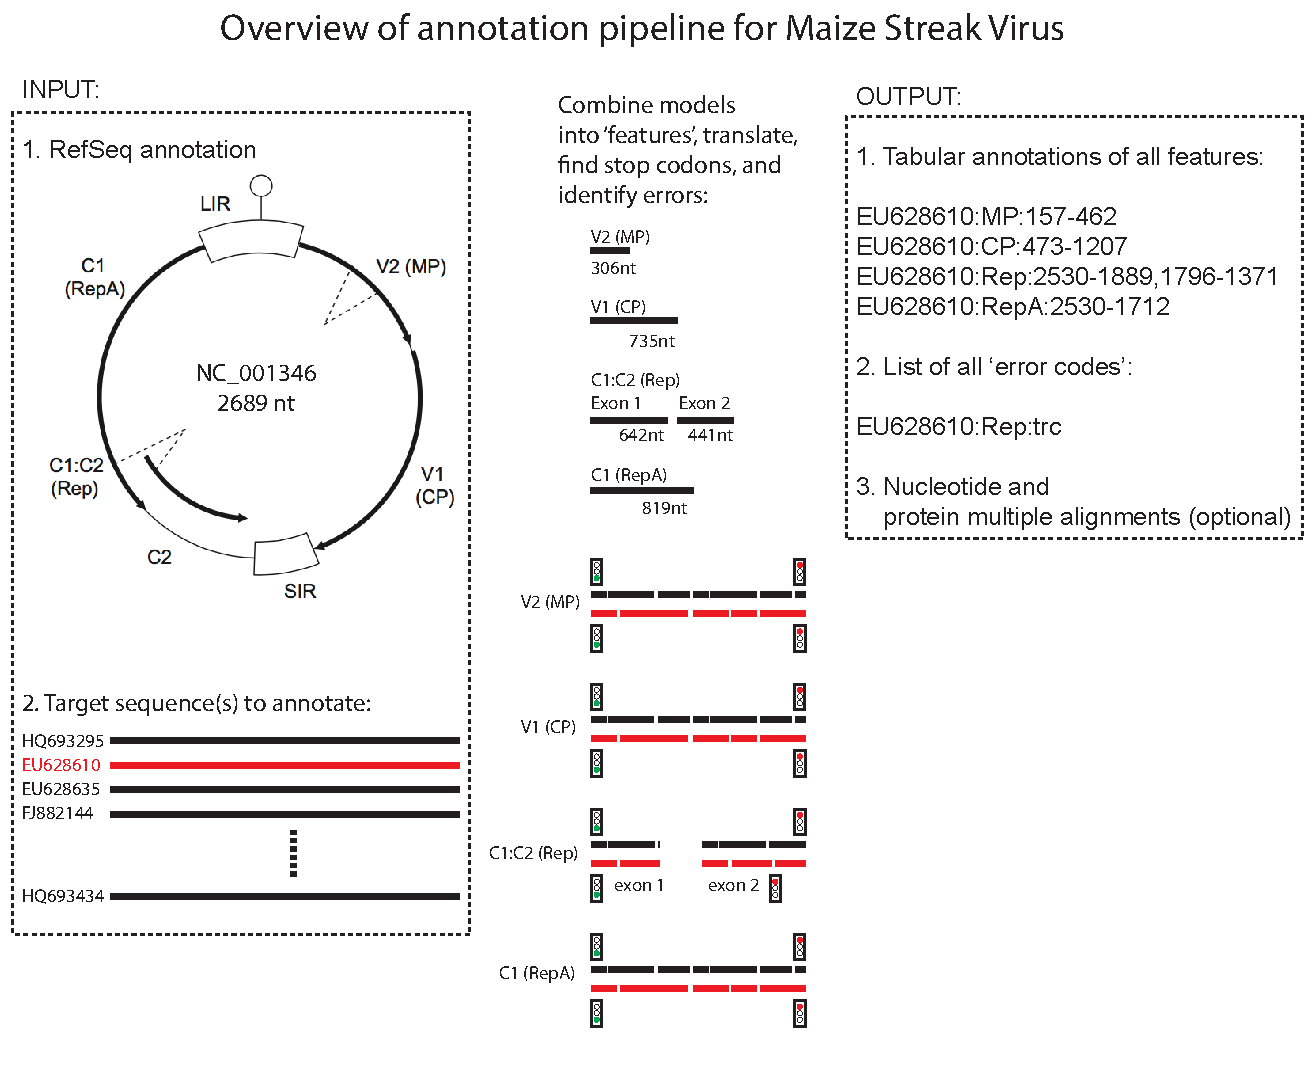
\includegraphics[width=10in]{figs/annotation-schematic-msv-4}
\vfill
\end{slide}
%%%%%%%%%%%%%%%%%%%%%%%%%%%%%%%%%%%%%%%%%%%%%%%%%%%%%%%%%%%%%%%%%%%%%%
\begin{slide}
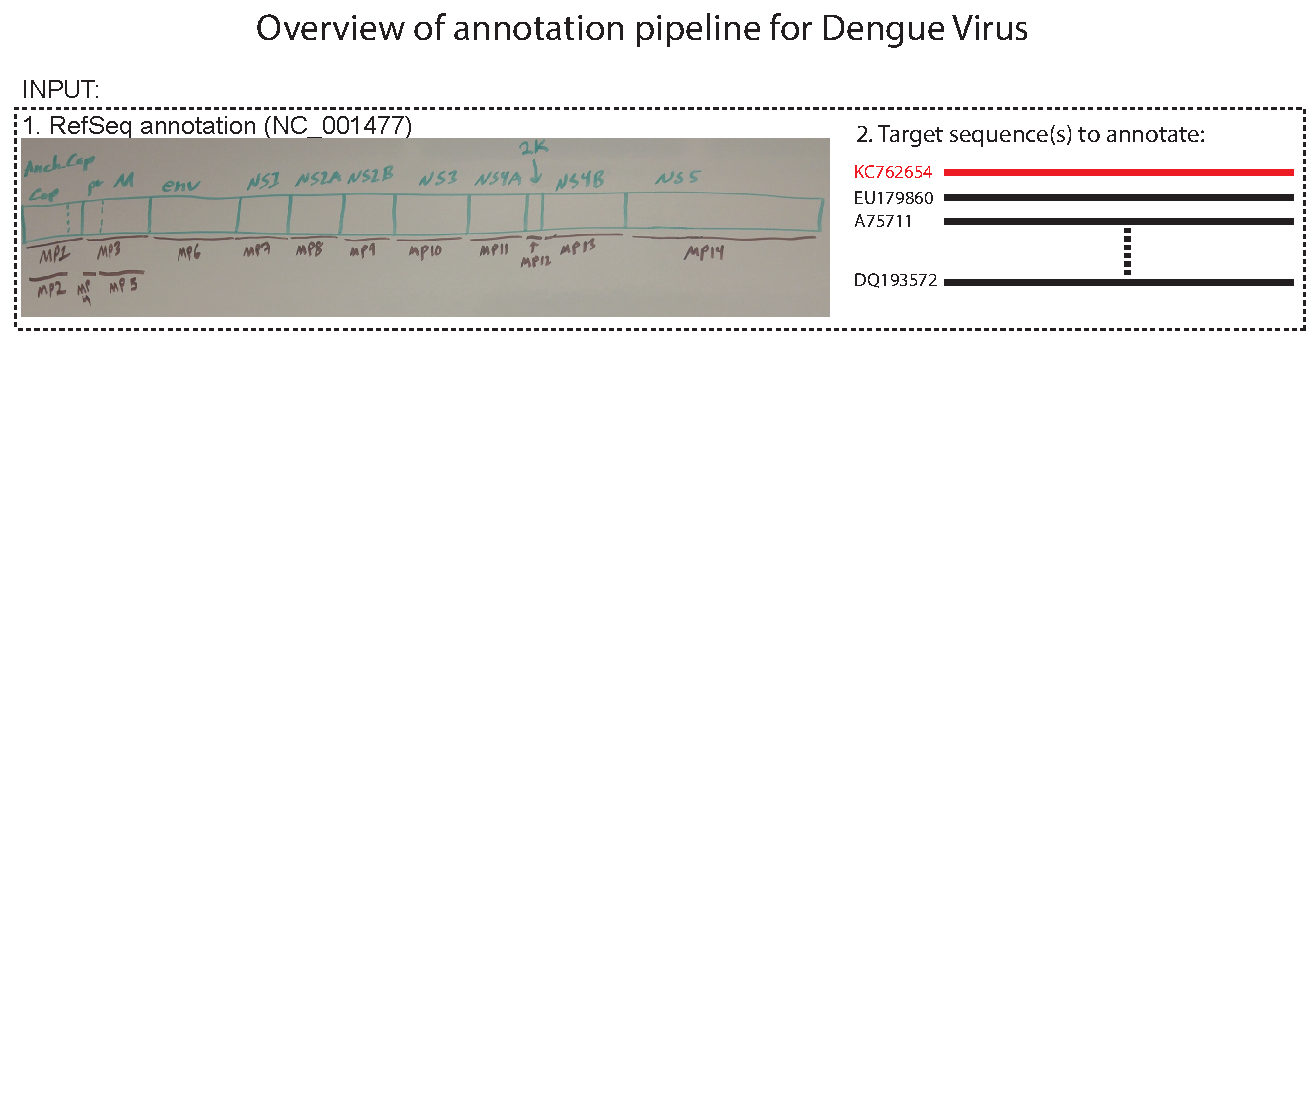
\includegraphics[width=10in]{figs/annotation-schematic-dengue-1}
\vfill
\end{slide}
%%%%%%%%%%%%%%%%%%%%%%%%%%%%%%%%%%%%%%%%%%%%%%%%%%%%%%%%%%%%%%%%%%%%%%
\begin{slide}
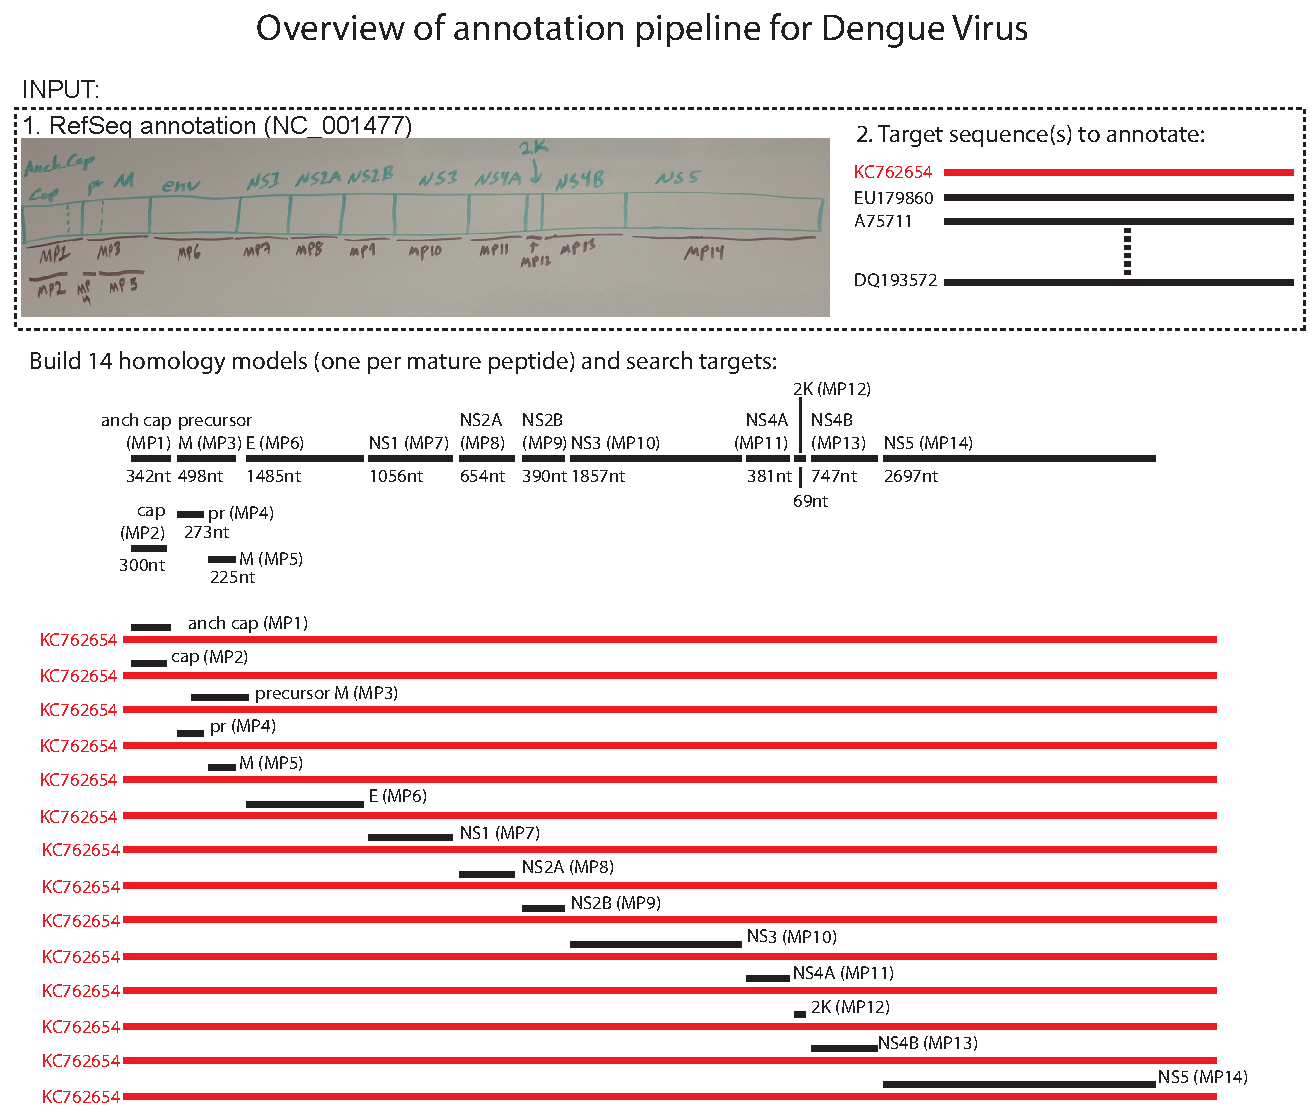
\includegraphics[width=10in]{figs/annotation-schematic-dengue-2}
\vfill
\end{slide}
%%%%%%%%%%%%%%%%%%%%%%%%%%%%%%%%%%%%%%%%%%%%%%%%%%%%%%%%%%%%%%%%%%%%%%
\begin{slide}
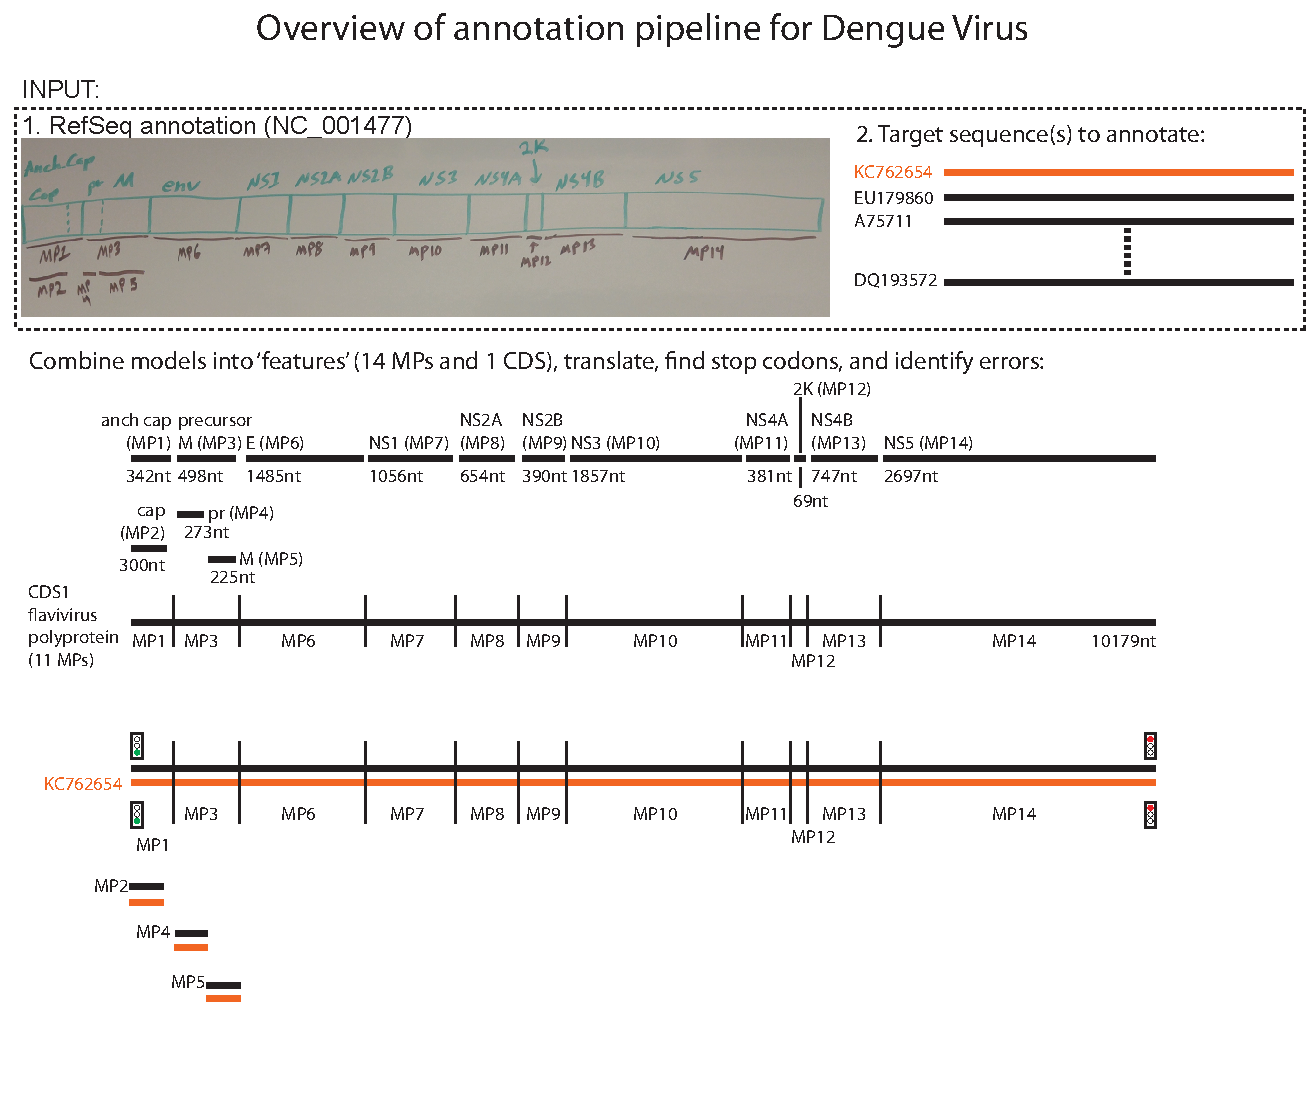
\includegraphics[width=10in]{figs/annotation-schematic-dengue-3}
\vfill
\end{slide}
%%%%%%%%%%%%%%%%%%%%%%%%%%%%%%%%%%%%%%%%%%%%%%%%%%%%%%%%%%%%%%%%%%%%%%
\begin{slide}
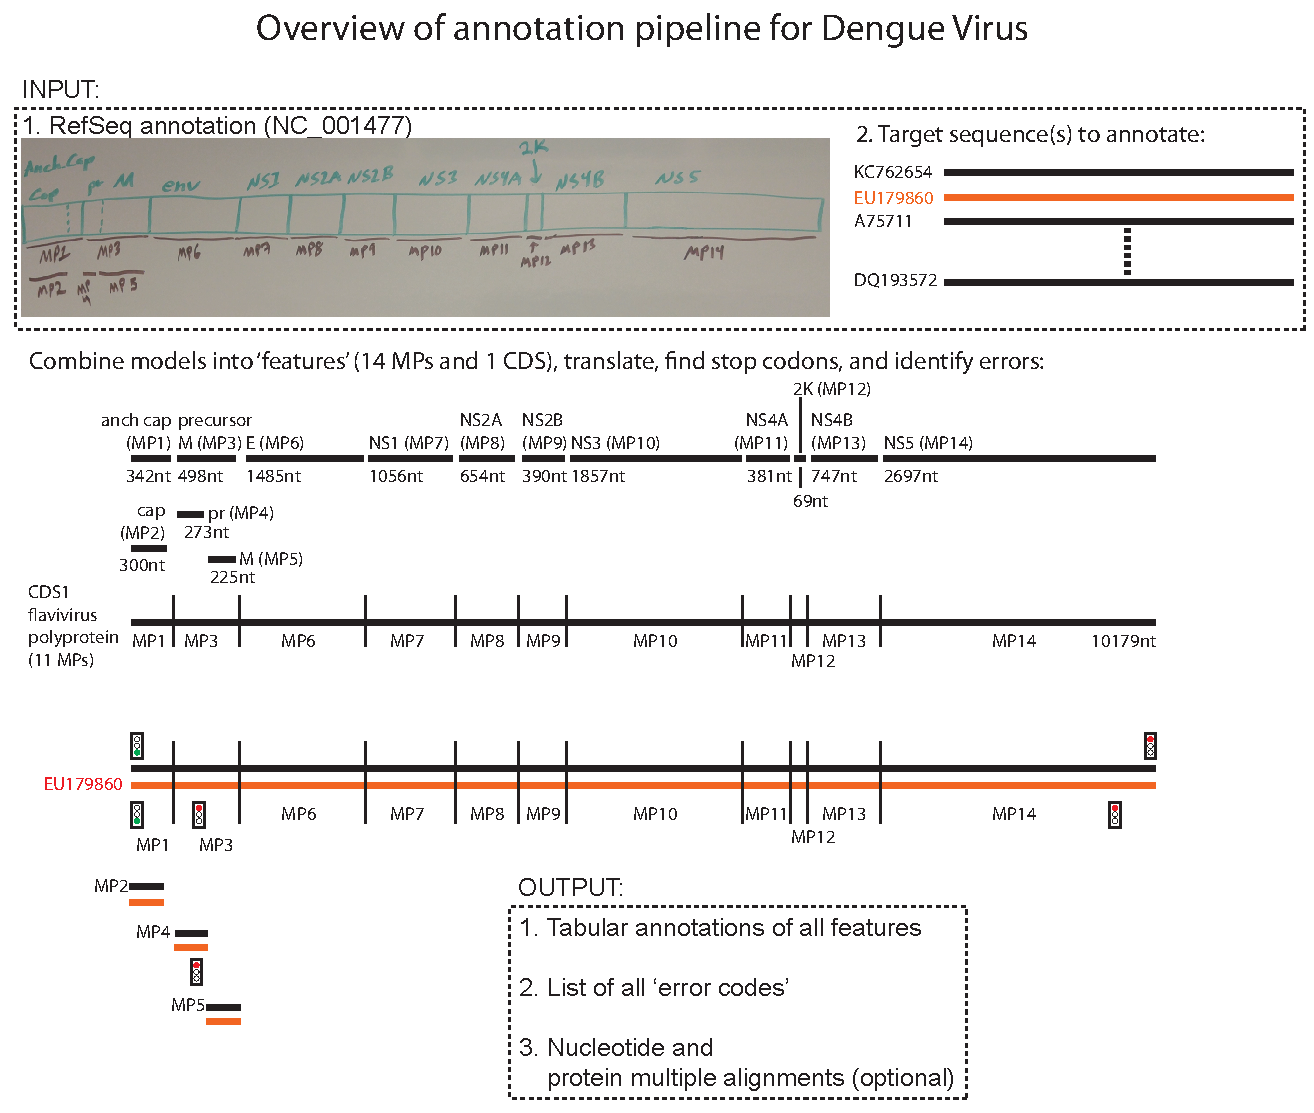
\includegraphics[width=10in]{figs/annotation-schematic-dengue-4-with-output}
\vfill
\end{slide}
%%%%%%%%%%%%%%%%%%%%%%%%%%%%%%%%%%%%%%%%%%%%%%%%%%%%%%%%%%%%%%%%%%%%%%
\begin{slide}

Error code schematic slides (TOFINISH)

\vfill
\end{slide}
%%%%%%%%%%%%%%%%%%%%%%%%%%%%%%%%%%%%%%%%%%%%%%%%%%%%%%%%%%%%%%%%%%%%%%
\begin{slide}

Pilot stats (table?)
\begin{itemize}
\item number of genomes
\item number with 0 errors
\item number of each error code
\item number of annotations that agree with GenBank (absent from GenBank)
\end{itemize}

\vfill
\end{slide}
%%%%%%%%%%%%%%%%%%%%%%%%%%%%%%%%%%%%%%%%%%%%%%%%%%%%%%%%%%%%%%%%%%%%%%
\begin{slide}

Examples of errors module (TODO)
\vfill
\end{slide}
%%%%%%%%%%%%%%%%%%%%%%%%%%%%%%%%%%%%%%%%%%%%%%%%%%%%%%%%%%%%%%%%%%%%%%
%%%%%%%%%%%%%%%%%%%%%%%%%%%%%%%%%%%%%%%%%%%%%%%%%%%%%%%%%%%%%%%%%%%%%%
\begin{slide}

Actual code module (TOFINISH)
\vfill
\end{slide}
%%%%%%%%%%%%%%%%%%%%%%%%%%%%%%%%%%%%%%%%%%%%%%%%%%%%%%%%%%%%%%%%%%%%%%
\begin{slide}
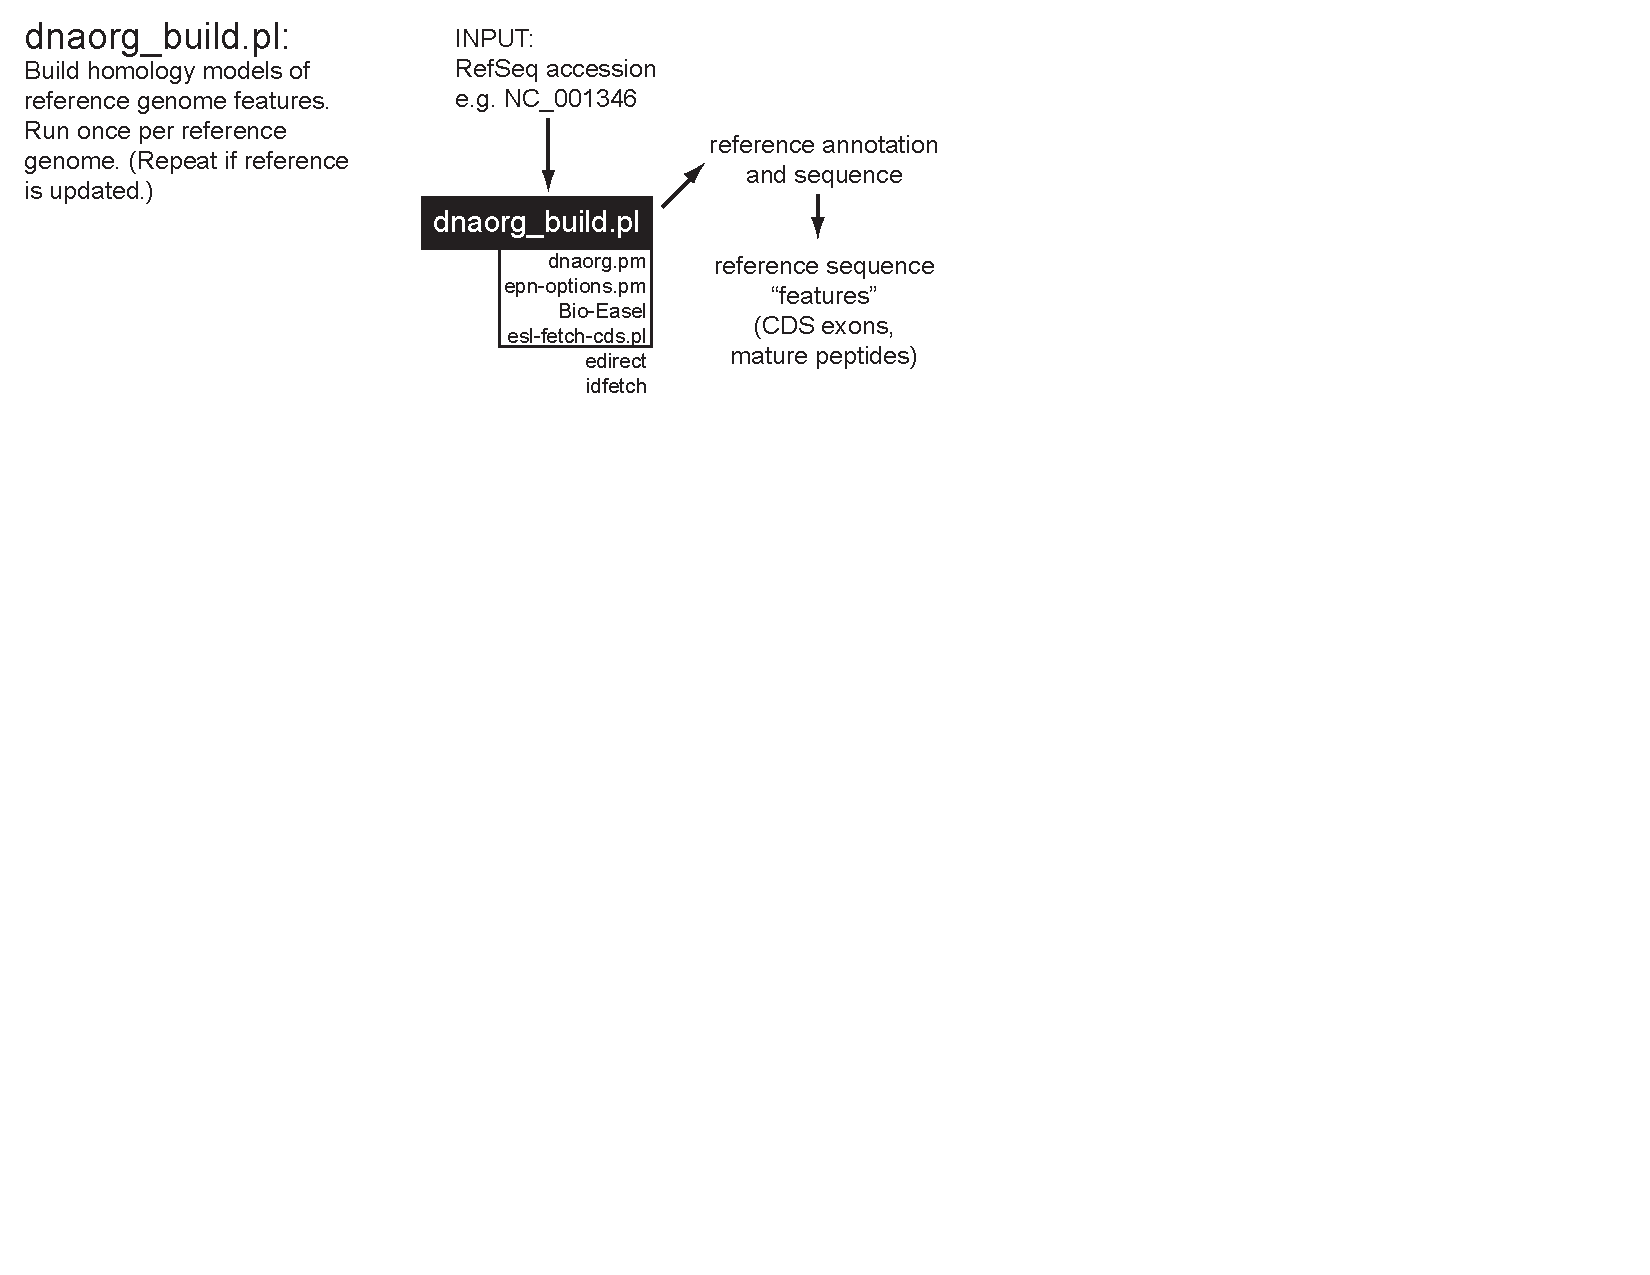
\includegraphics[width=10in]{figs/dnaorg-scripts-build1}
\vfill
\end{slide}
%%%%%%%%%%%%%%%%%%%%%%%%%%%%%%%%%%%%%%%%%%%%%%%%%%%%%%%%%%%%%%%%%%%%%%
\begin{slide}
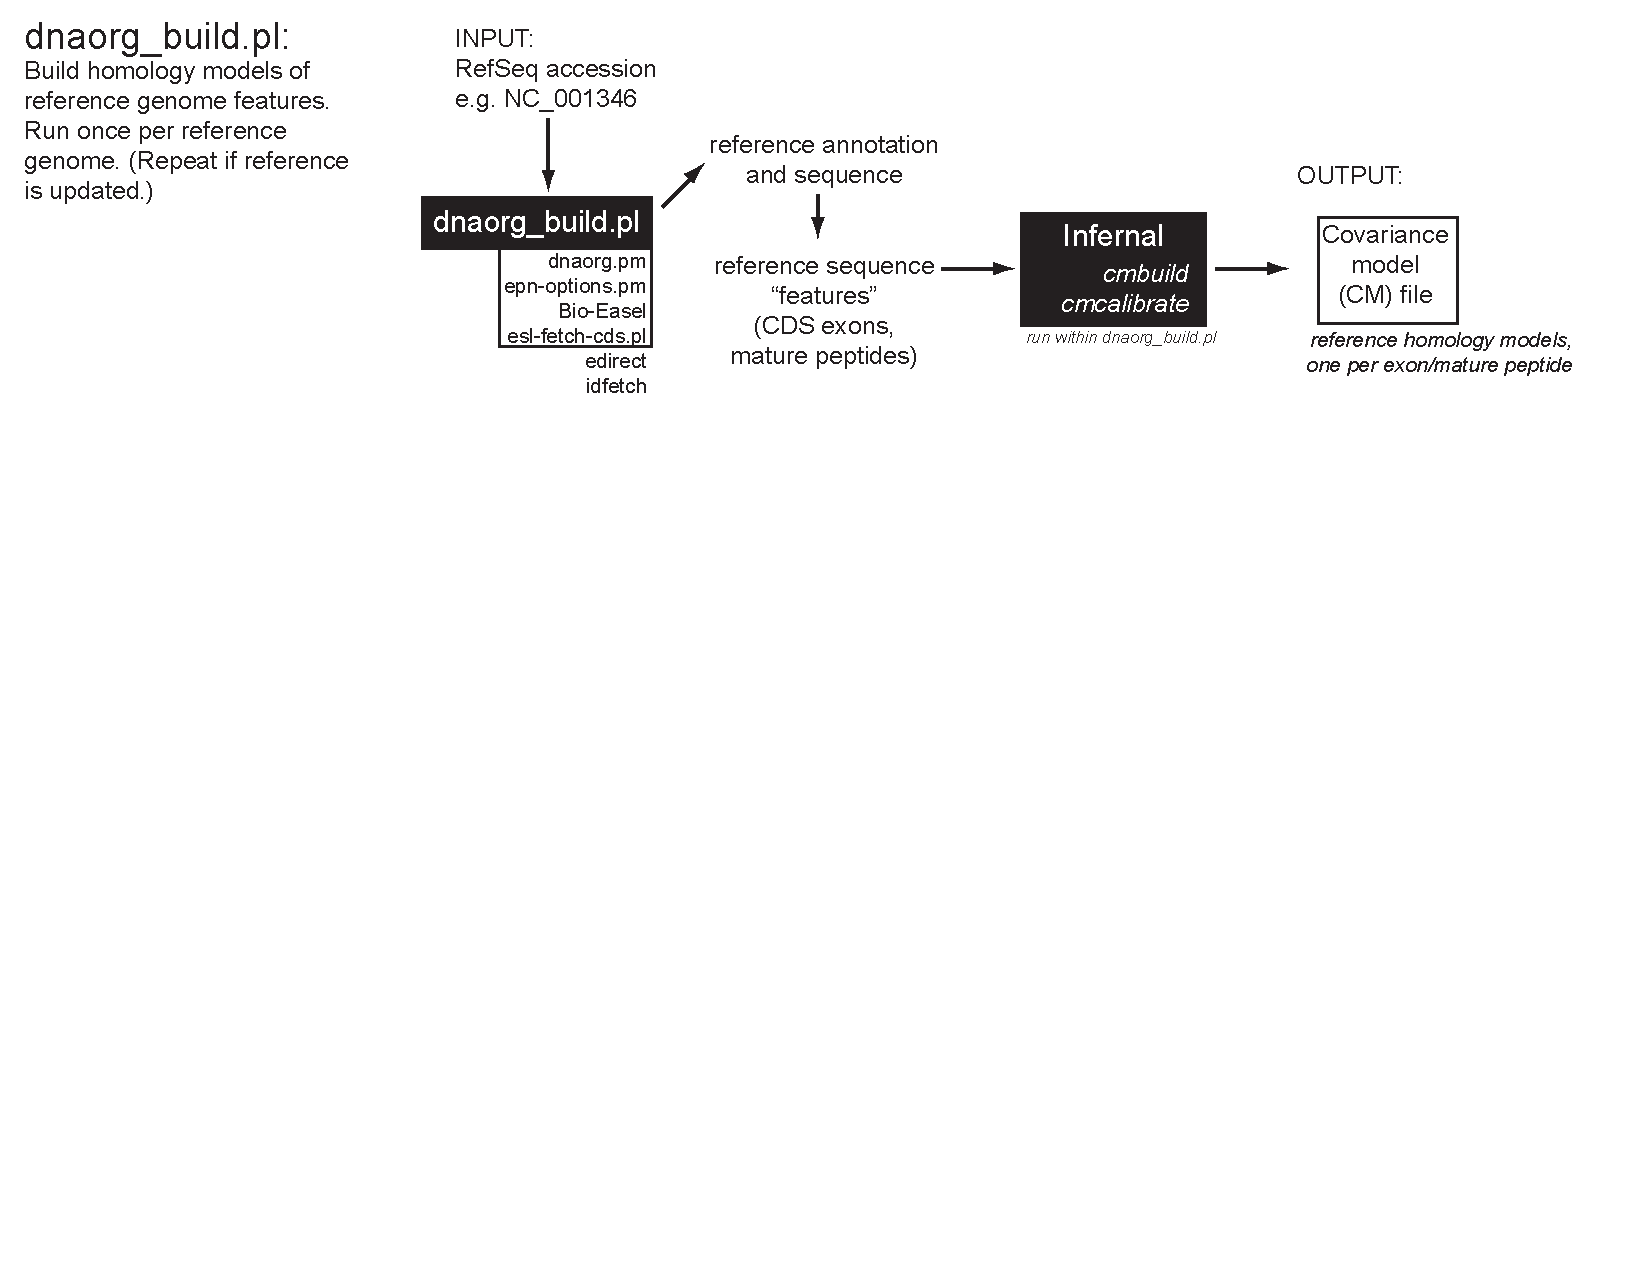
\includegraphics[width=10in]{figs/dnaorg-scripts-build2}
\vfill
\end{slide}
%%%%%%%%%%%%%%%%%%%%%%%%%%%%%%%%%%%%%%%%%%%%%%%%%%%%%%%%%%%%%%%%%%%%%%
\begin{slide}
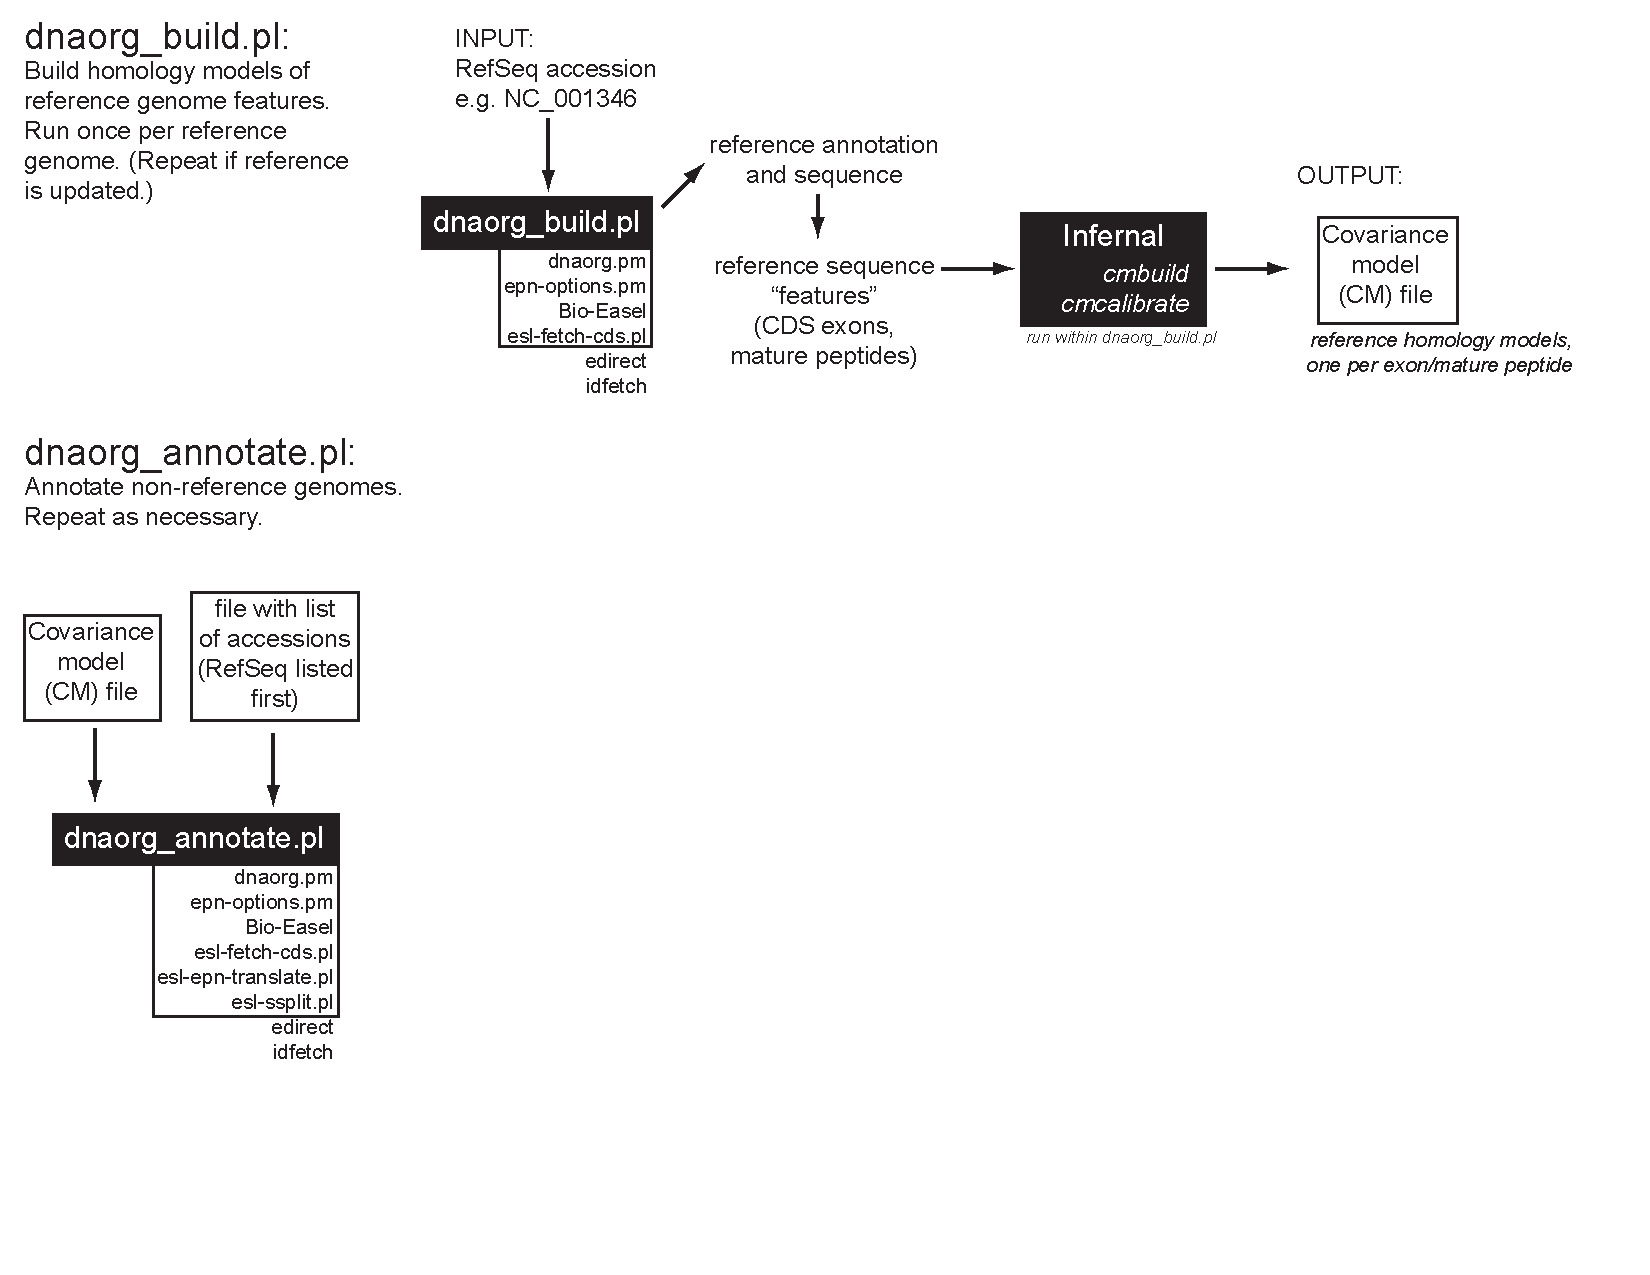
\includegraphics[width=10in]{figs/dnaorg-scripts-annotate1}
\vfill
\end{slide}
%%%%%%%%%%%%%%%%%%%%%%%%%%%%%%%%%%%%%%%%%%%%%%%%%%%%%%%%%%%%%%%%%%%%%%
\begin{slide}
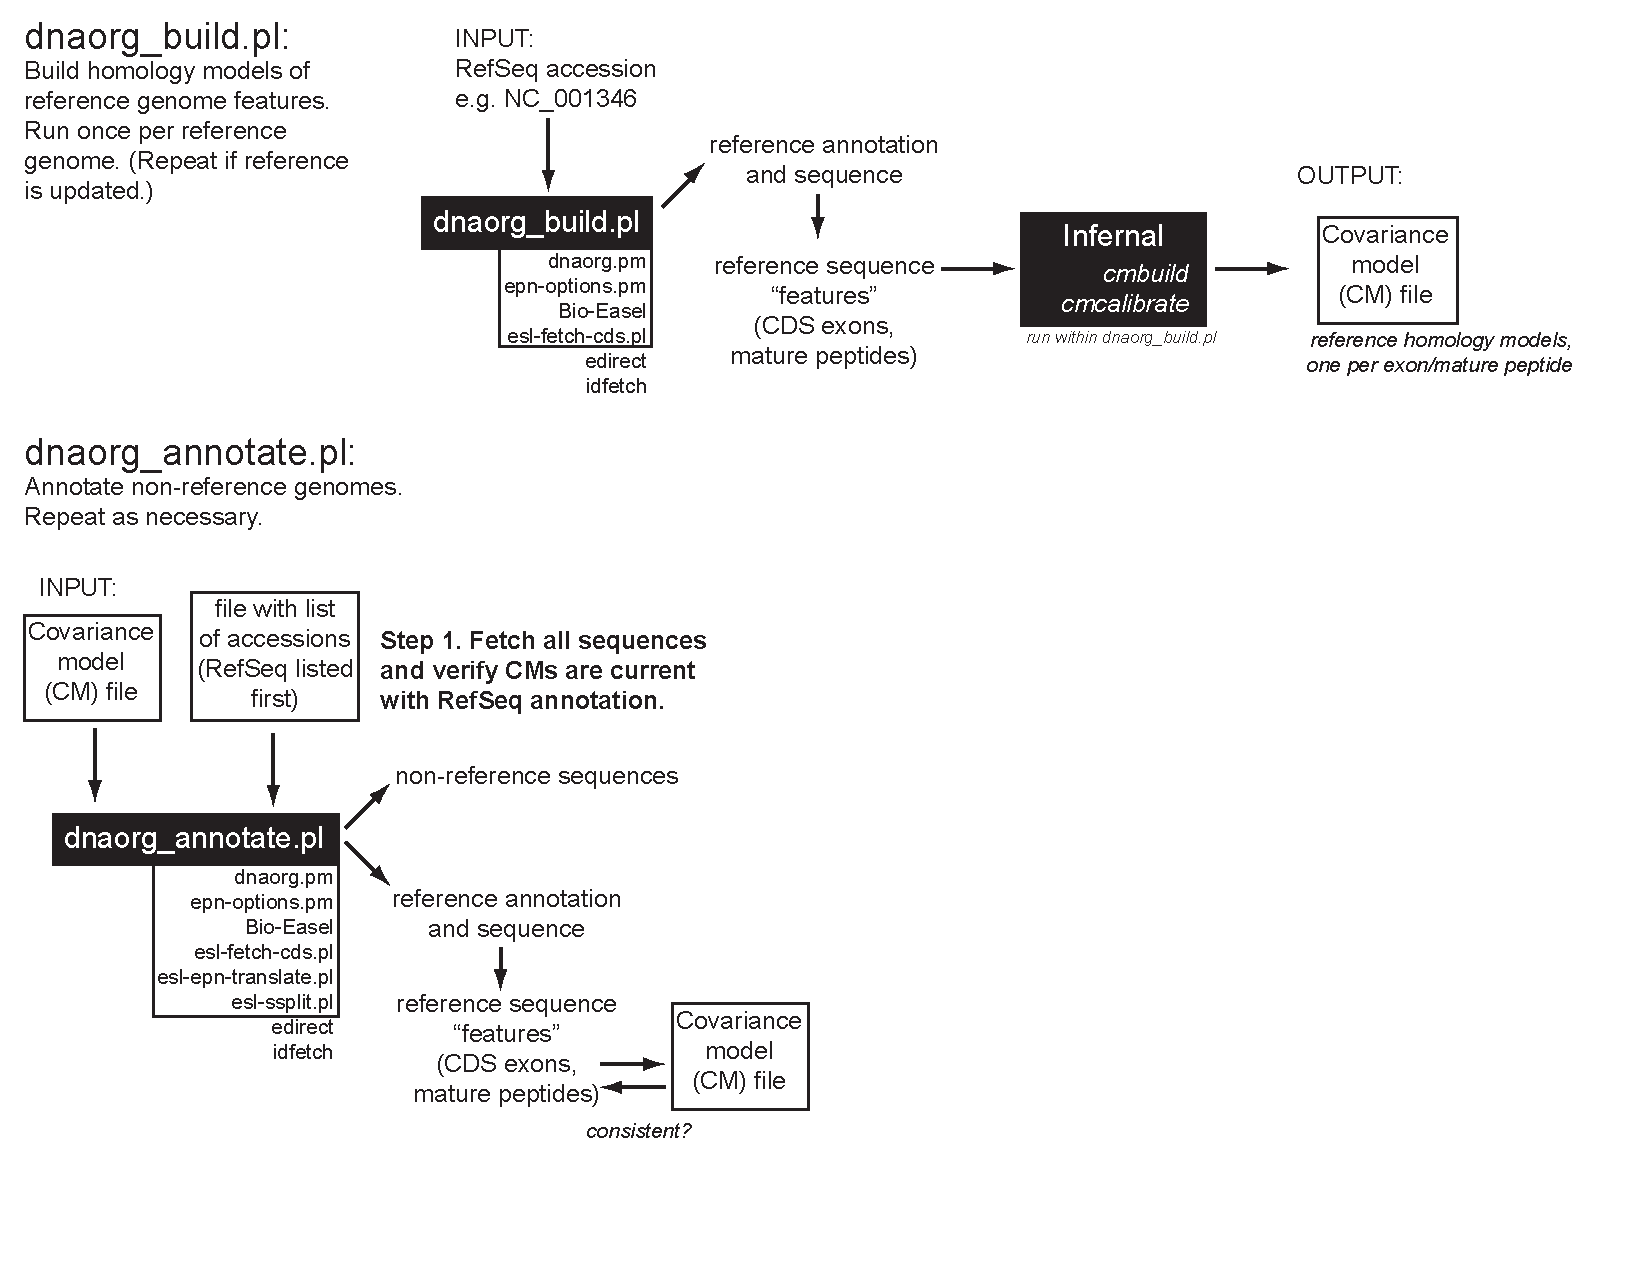
\includegraphics[width=10in]{figs/dnaorg-scripts-annotate2}
\vfill
\end{slide}
%%%%%%%%%%%%%%%%%%%%%%%%%%%%%%%%%%%%%%%%%%%%%%%%%%%%%%%%%%%%%%%%%%%%%%
\begin{slide}
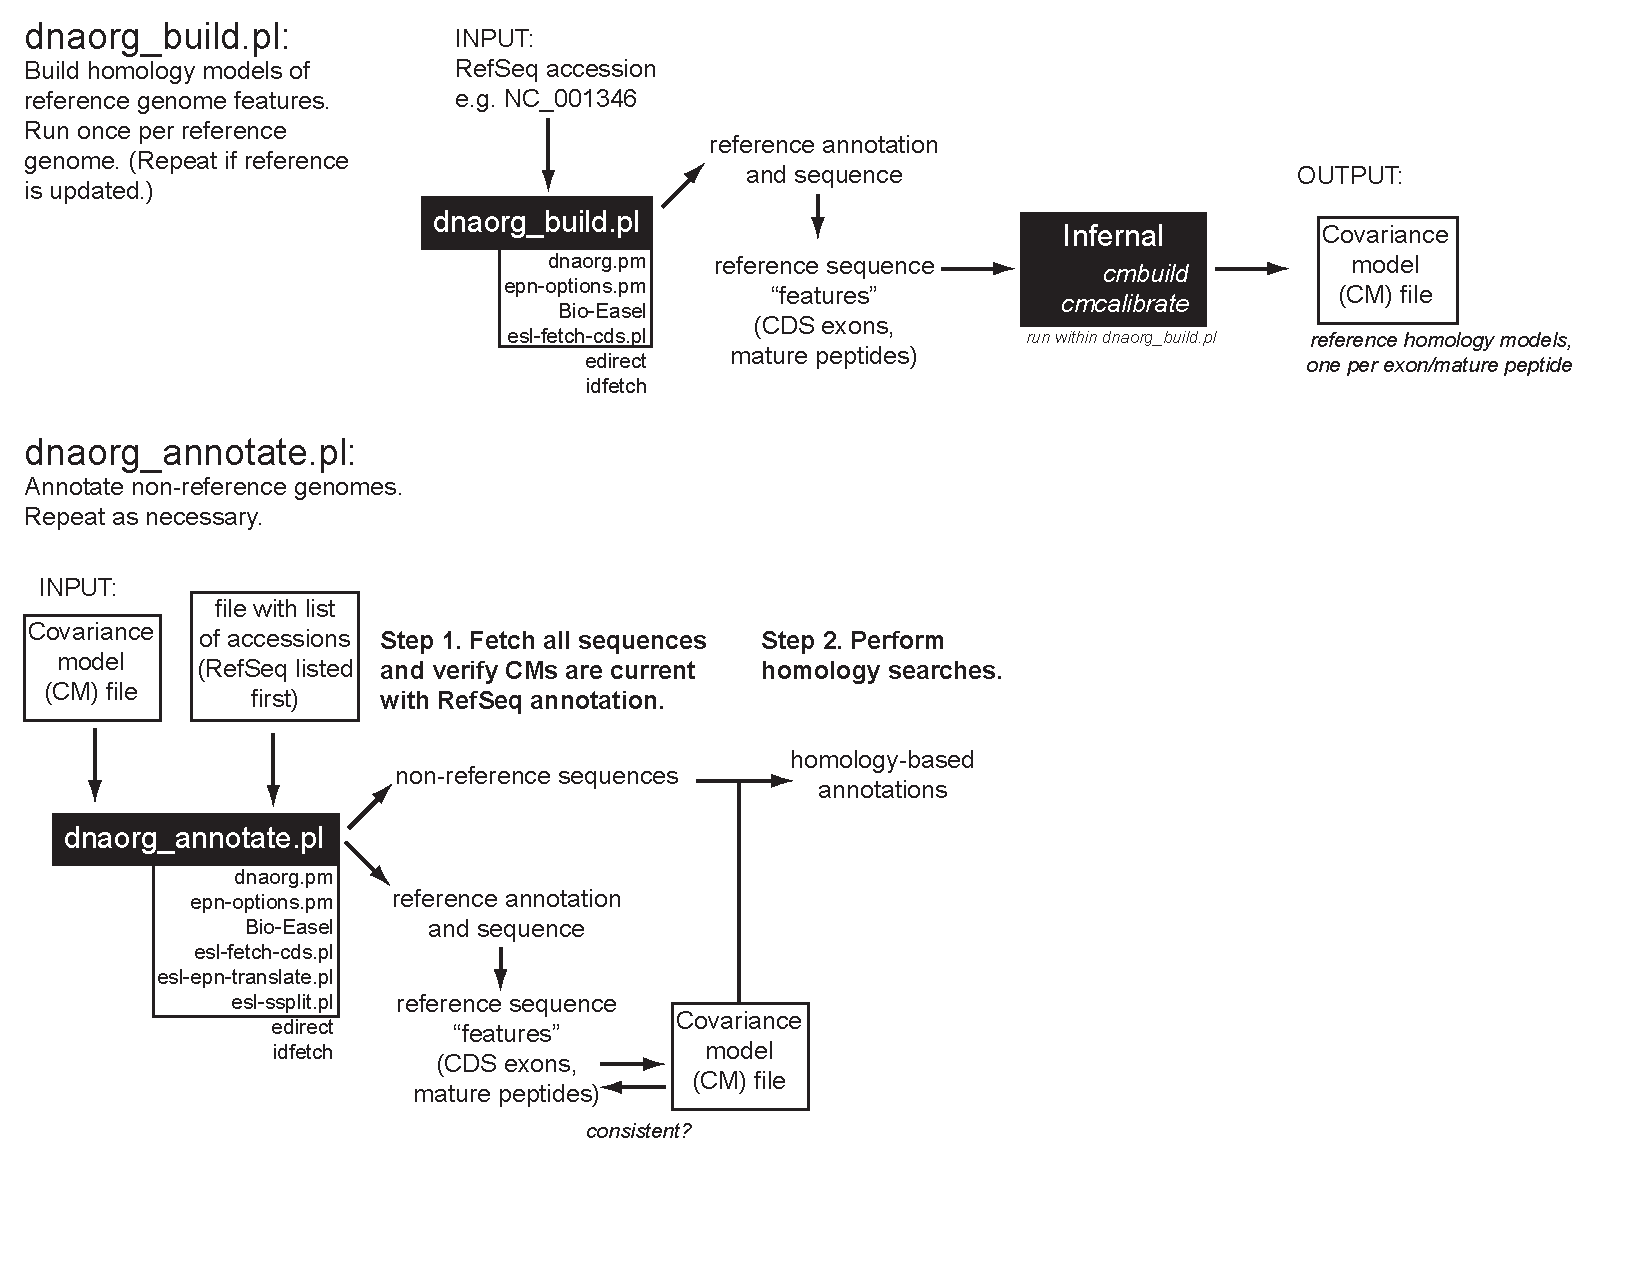
\includegraphics[width=10in]{figs/dnaorg-scripts-annotate3}
\vfill
\end{slide}
%%%%%%%%%%%%%%%%%%%%%%%%%%%%%%%%%%%%%%%%%%%%%%%%%%%%%%%%%%%%%%%%%%%%%%
\begin{slide}
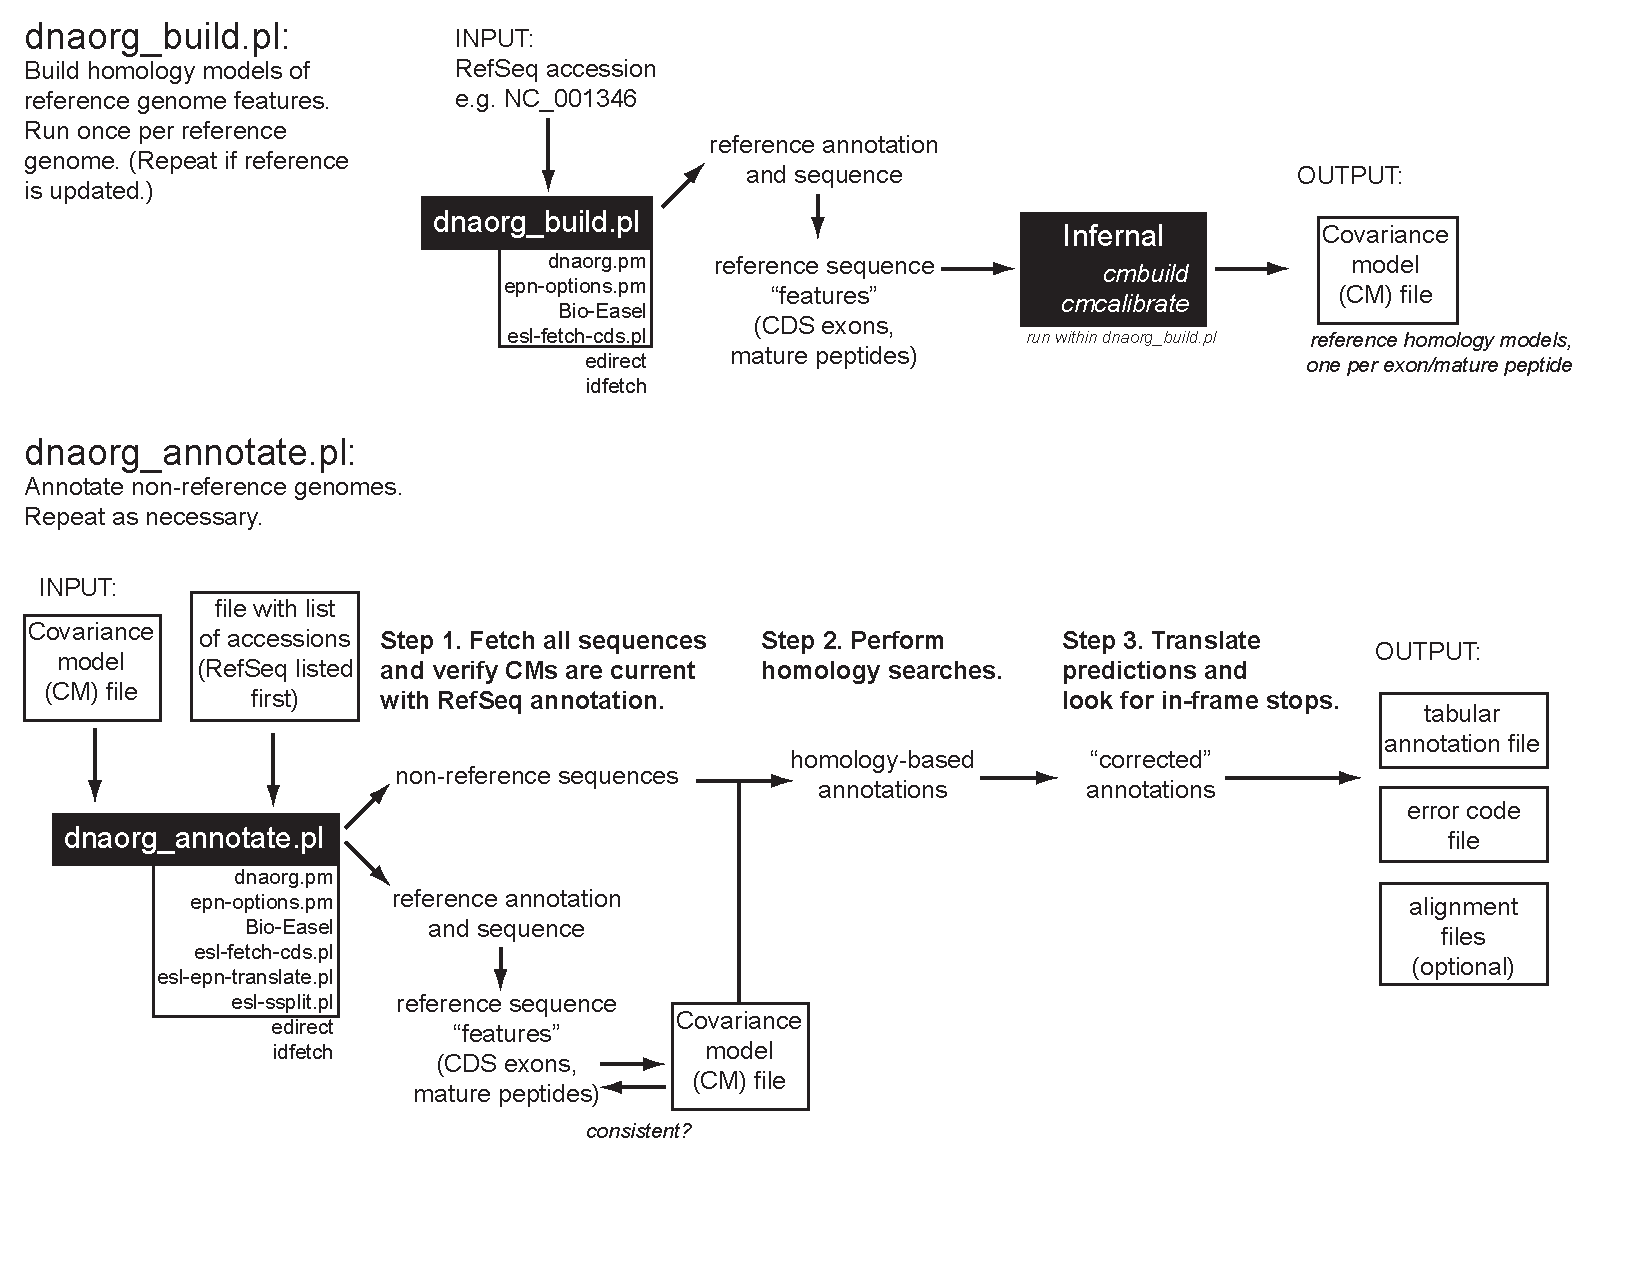
\includegraphics[width=10in]{figs/dnaorg-scripts-annotate4}
\vfill
\end{slide}
%%%%%%%%%%%%%%%%%%%%%%%%%%%%%%%%%%%%%%%%%%%%%%%%%%%%%%%%%%%%%%%%%%%%%%
\begin{slide}
\begin{center}
\textbf{Annotating Maize Streak Virus: dnaorg\_build.pl step} 

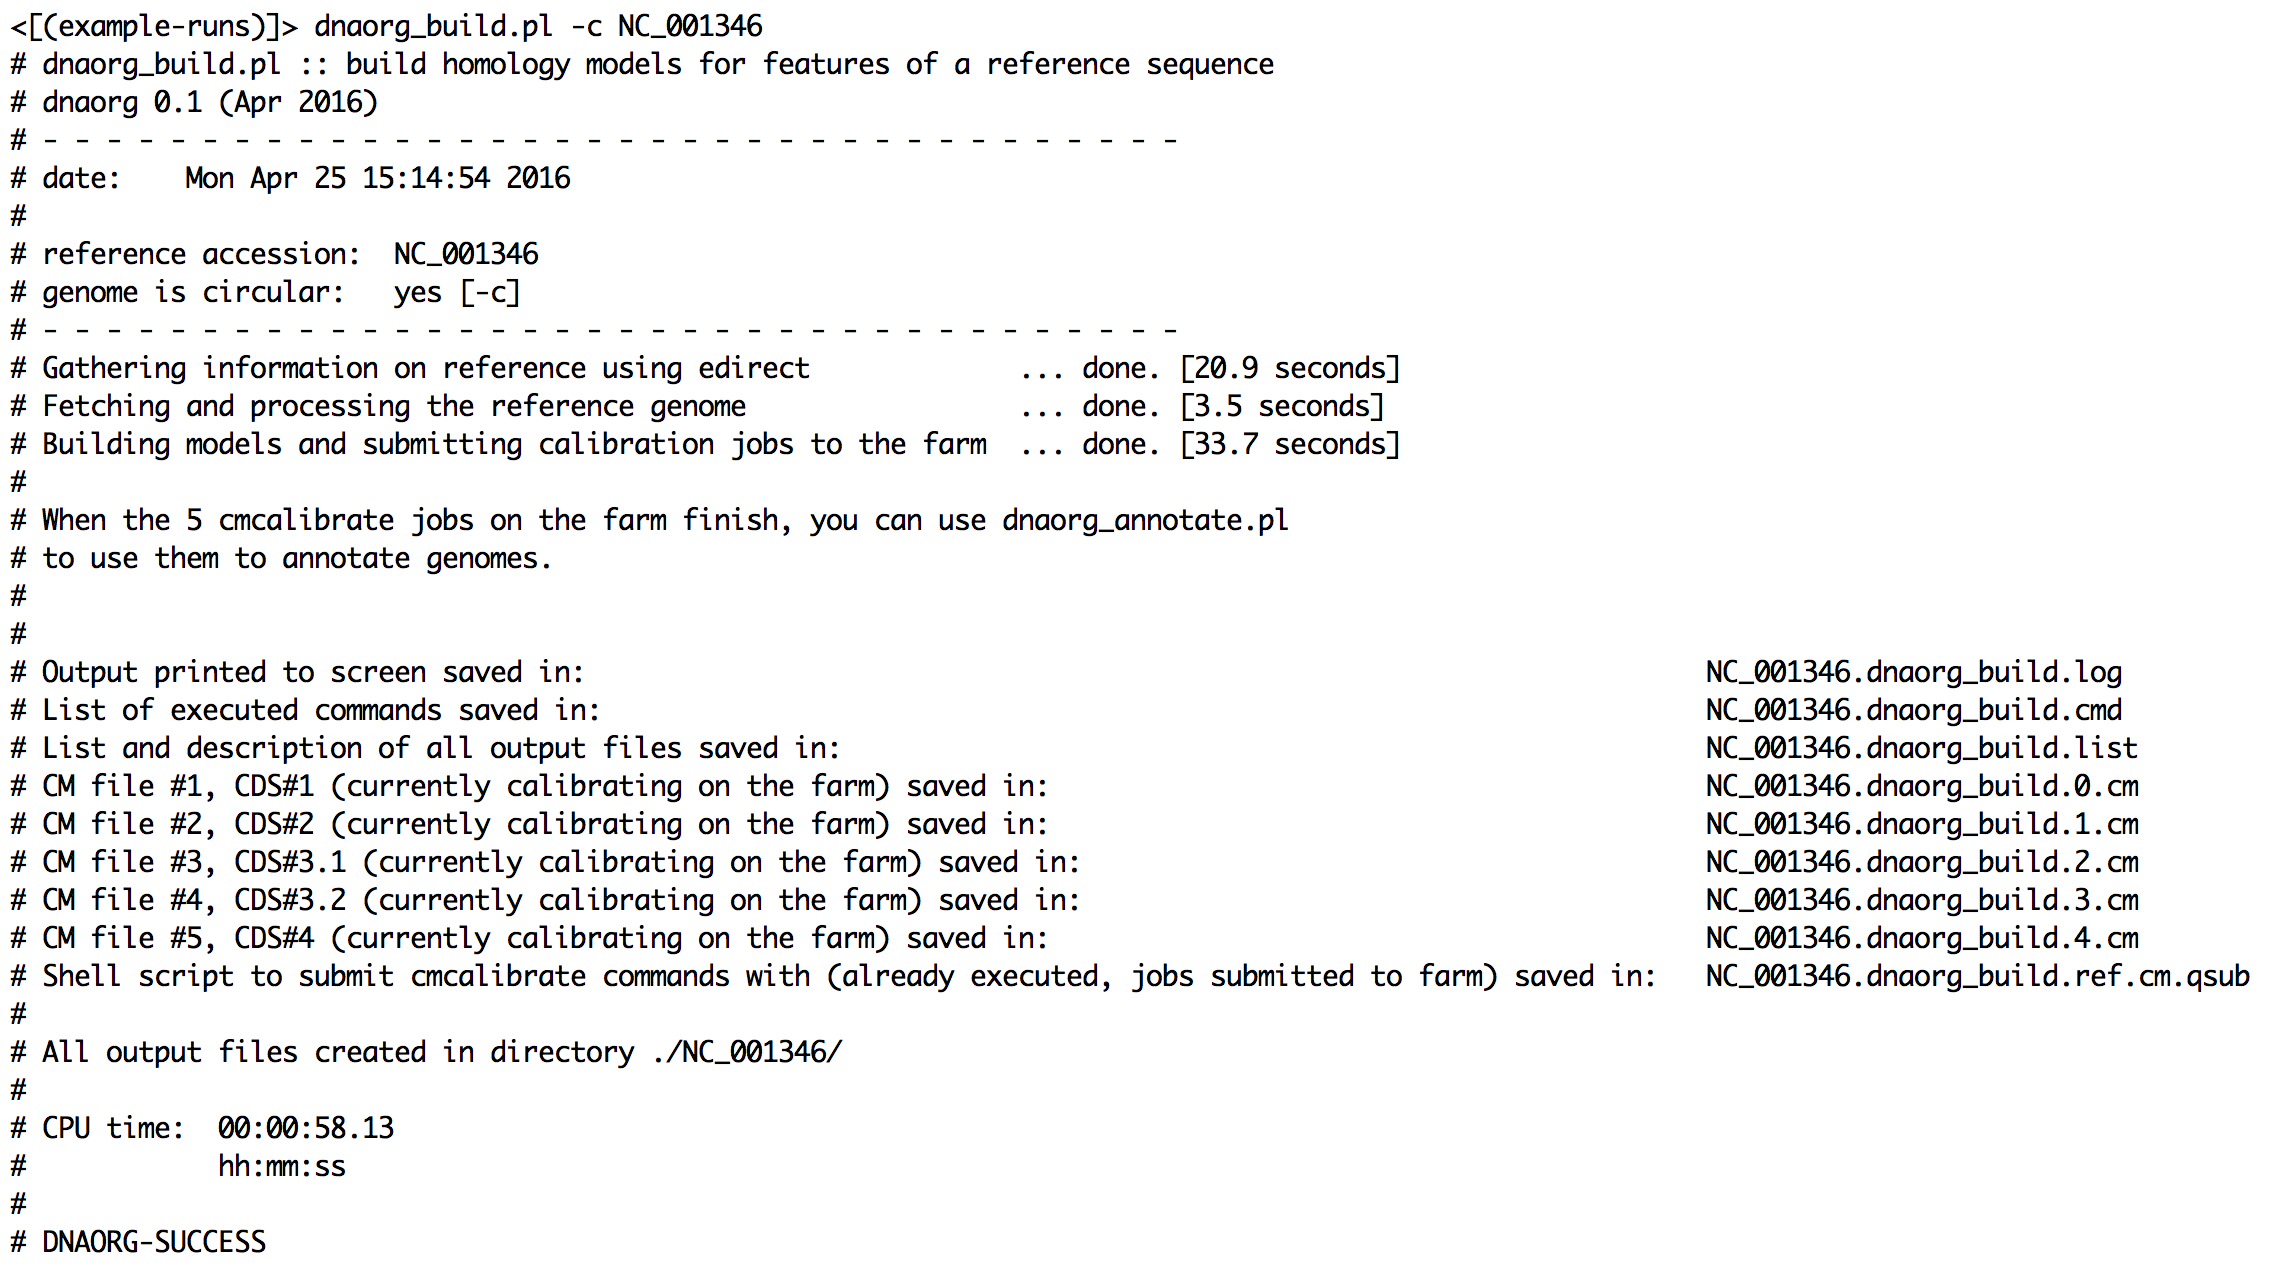
\includegraphics[width=8in]{figs/dnaorg-build-output}

\end{center}
\vfill
\end{slide}
%%%%%%%%%%%%%%%%%%%%%%%%%%%%%%%%%%%%%%%%%%%%%%%%%%%%%%%%%%%%%%%%%%%%%%
\begin{slide}
\begin{center}
\textbf{Annotating Maize Streak Virus: dnaorg\_annotate.pl step} 

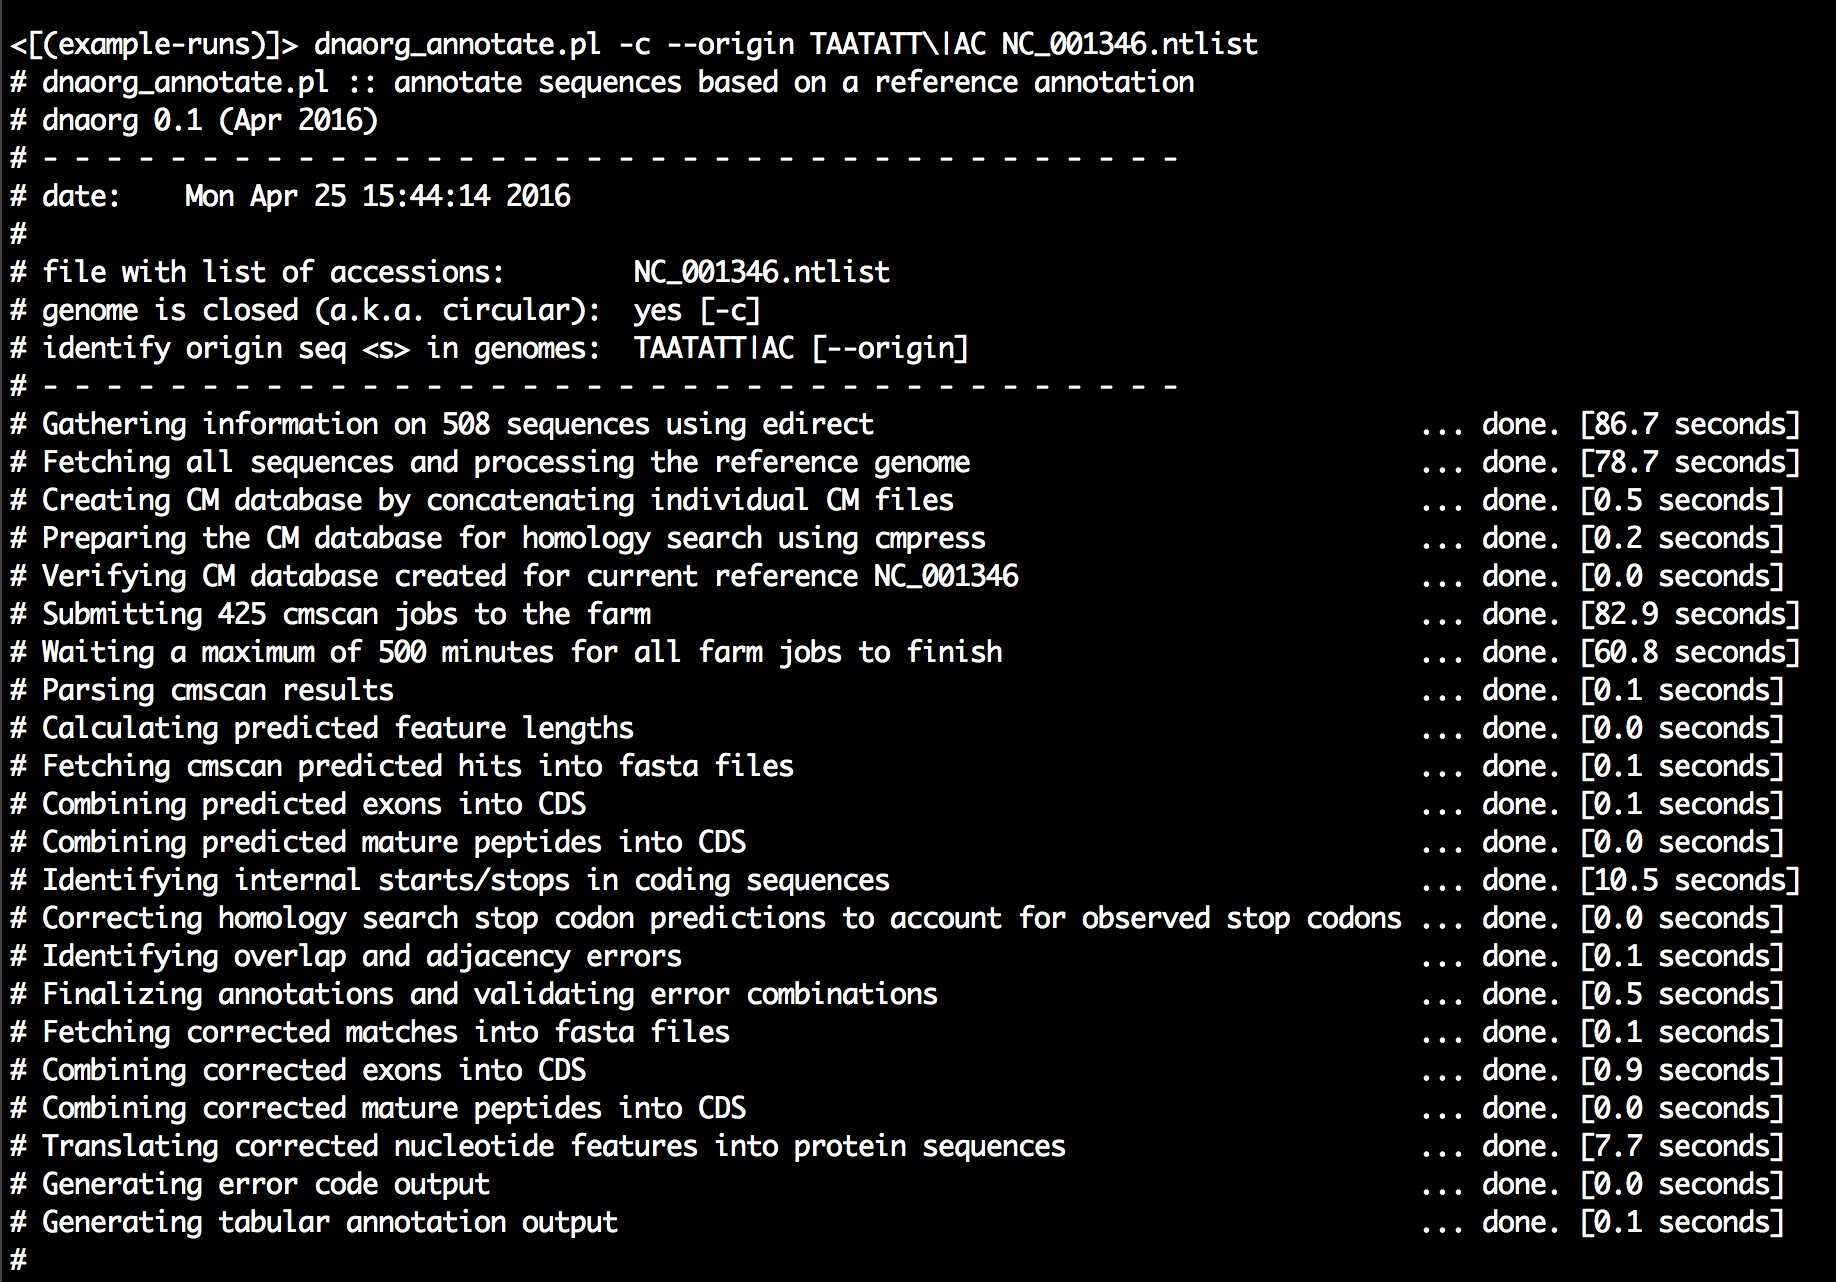
\includegraphics[width=8in]{figs/dnaorg-annotate-output1}

\end{center}
\vfill
\end{slide}
%%%%%%%%%%%%%%%%%%%%%%%%%%%%%%%%%%%%%%%%%%%%%%%%%%%%%%%%%%%%%%%%%%%%%%
\begin{slide}
\begin{center}
\textbf{Annotating Maize Streak Virus: dnaorg\_annotate.pl step} 

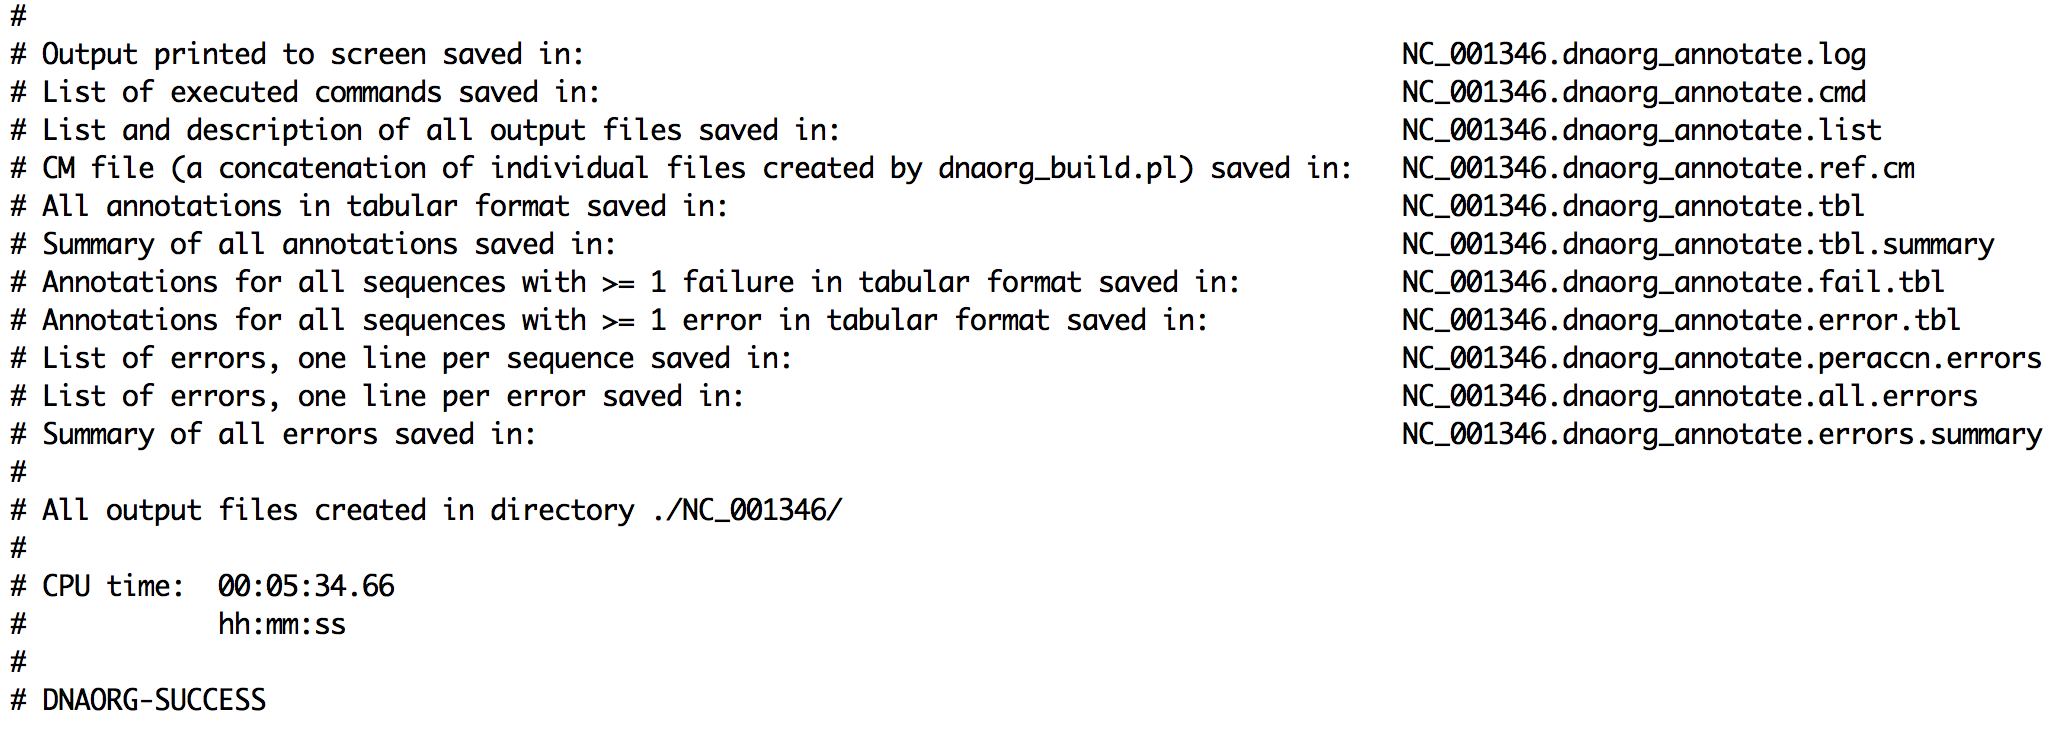
\includegraphics[width=8in]{figs/dnaorg-annotate-output2}

\end{center}
\vfill
\end{slide}
%%%%%%%%%%%%%%%%%%%%%%%%%%%%%%%%%%%%%%%%%%%%%%%%%%%%%%%%%%%%%%%%%%%%%%
\begin{slide}
\begin{center}
\textbf{Annotating Maize Streak Virus: dnaorg\_annotate.pl step} 

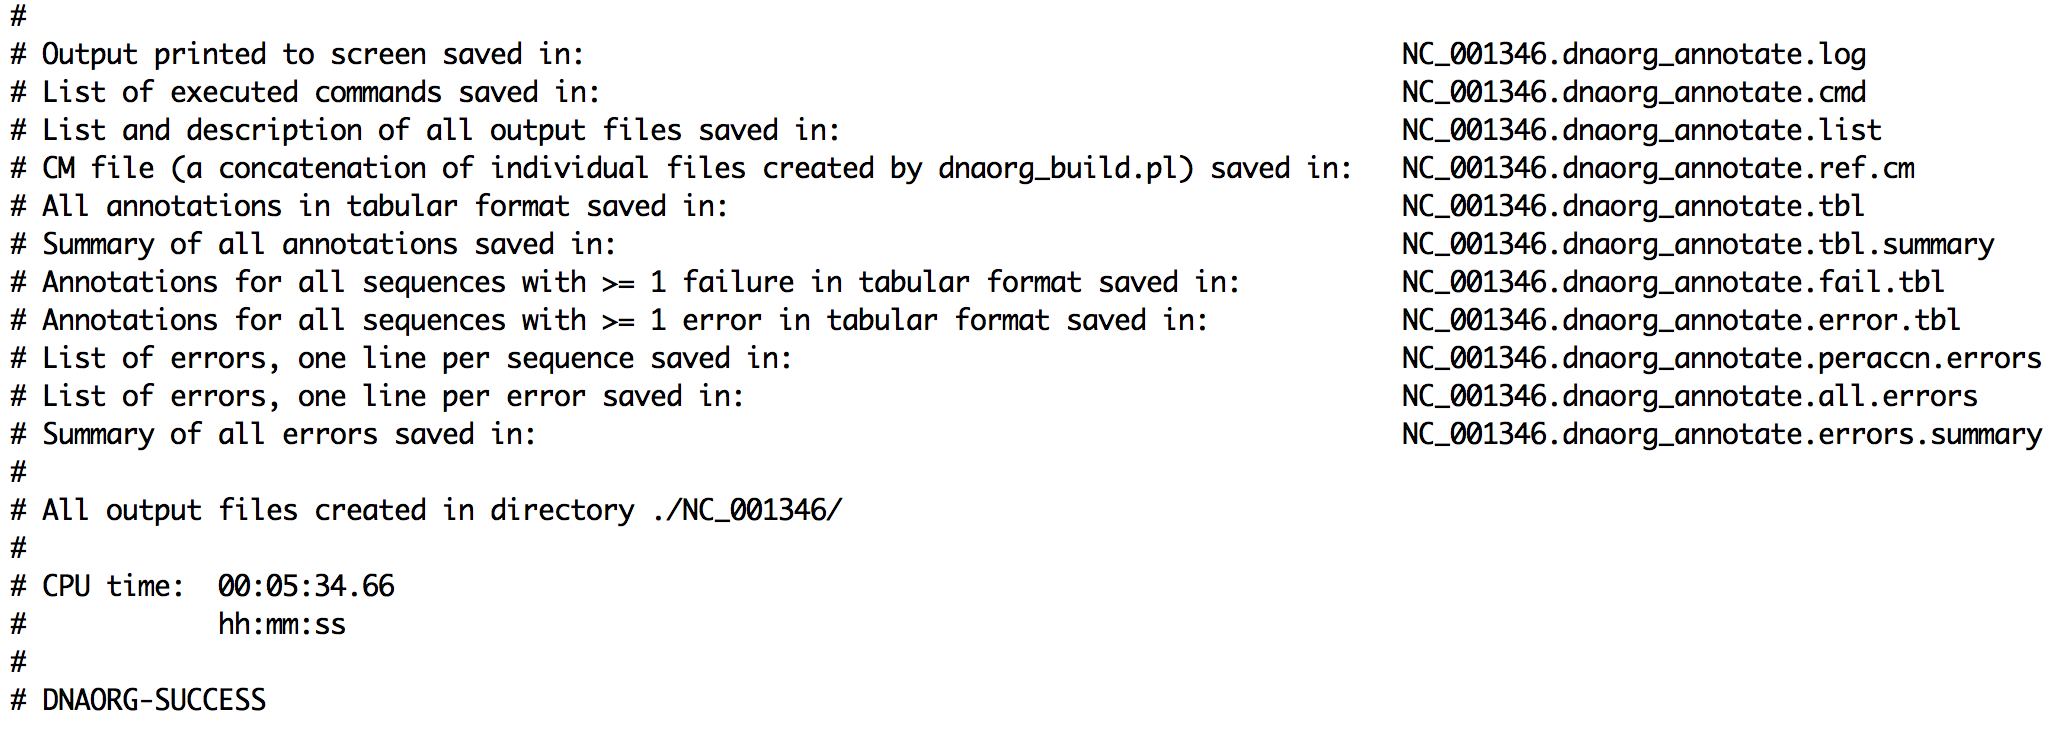
\includegraphics[width=8in]{figs/dnaorg-annotate-output3}

\end{center}
\vfill
\end{slide}
%%%%%%%%%%%%%%%%%%%%%%%%%%%%%%%%%%%%%%%%%%%%%%%%%%%%%%%%%%%%%%%%%%%%%%
\begin{slide}
\textbf{Infernal was chosen for homology search tool because it
  encourages global alignment}

\begin{itemize}
\item Maybe this slide should go at end? 
\end{itemize}

\vfill
\end{slide}
%%%%%%%%%%%%%%%%%%%%%%%%%%%%%%%%%%%%%%%%%%%%%%%%%%%%%%%%%%%%%%%%%%%%%%
\begin{slide}
\textbf{Future directions module (TODO)}

\vfill
\end{slide}
%%%%%%%%%%%%%%%%%%%%%%%%%%%%%%%%%%%%%%%%%%%%%%%%%%%%%%%%%%%%%%%%%%%%%%

\end{document}
